\chapter{Materiali e metodi}
\label{cap:metodi}

Questo capitolo descrive i materiali, l'architettura e il metodo di verifica della pipeline di ingestion sviluppata nella tesi. La descrizione e la valutazione si basano su tre fonti complementari: il codice del pacchetto \texttt{manual\_ingestion} e i test ne definiscono e verificano il comportamento; la documentazione ricostruisce le scelte progettuali e le prove di accettazione; i bundle e le registrazioni delle due esecuzioni finali di enrichment del 15 settembre 2026 consentono di controllare gli ingressi e le uscite di quel ciclo sperimentale.

Il progetto separa la distribuzione del software dai materiali dello studio. La repository pubblica \path{industrial-manual-ingestion} contiene il prodotto finale; il workspace privato \path{tesi-di-nardo} raccoglie il diario delle decisioni, le matrici di accettazione, le run V4 e i materiali di valutazione. È una distinzione organizzativa, che non modifica l'architettura della pipeline né il contratto del run bundle. Nel seguito, i riferimenti ai moduli sono relativi al pacchetto \texttt{manual\_ingestion}, collocato nella directory \path{src/manual_ingestion/} della repository pubblica.

Le sigle di versione indicano oggetti diversi: V2 designa l'architettura integrata del prodotto, mentre V3 e V4 identificano cicli dello studio di enrichment. Non corrispondono quindi al tag della release pubblica \texttt{v1.0.0}, né alla versione del pacchetto registrata nelle run o a quella dello schema documentale. Anche il prompt ha una propria versione: il ciclo V4 usa ancora \texttt{technical-caption-v3}.

\section{Caso applicativo, corpus e requisiti}

Il caso applicativo è la preparazione di manuali tecnici industriali per una successiva consultazione assistita, nel contesto delineato nel Capitolo~\ref{cap:introduzione}. L'unità di ingresso della pipeline è un PDF; l'unità di uscita è un insieme coordinato di artefatti, denominato \emph{run bundle}, che descrive sia il documento elaborato sia l'esecuzione che lo ha prodotto. Il confine del sistema precede il chunking: la pipeline non calcola embedding, non costruisce un indice vettoriale e non esegue retrieval o generazione di risposte.

L'eterogeneità degli ingressi è affrontata distinguendo tre condizioni operative: PDF con testo digitale e outline incorporato; PDF con testo digitale ma privi di outline; PDF con copertura testuale insufficiente, che richiedono OCR. Si tratta di condizioni rilevate dal programma, non di tre corpus indipendenti. In particolare, un PDF misto può essere instradato verso l'OCR anche se alcune pagine contengono testo estraibile. L'assenza di outline non implica inoltre che qualsiasi struttura sia ricostruibile: il percorso digitale senza segnalibri richiede un indice stampato riconoscibile.

L'implementazione risponde a quattro requisiti. Il primo è uniformare l'uscita dei parser senza perdere l'identità dei contenuti acquisiti. Il secondo è conservare la relazione tra elementi, pagine e capitoli, insieme alle coordinate quando disponibili. Il terzo è separare le informazioni estratte da quelle generate e rendere esplicite le esclusioni. Il quarto è pubblicare soltanto bundle tecnicamente coerenti, distinguendo quelli conformi alla politica di accettazione da quelli sperimentali. Il campo \texttt{include\_in\_rag} esprime una destinazione d'uso prevista, mentre l'indicizzazione dell'elemento appartiene al sistema a valle. A questi requisiti si affiancano l'esecuzione locale, l'assenza di fine-tuning e un output strutturato che non dipende dal sistema Django/RAG a valle, come documentato nel diario di progetto.

\subsection{Documenti e condizioni di ingresso}

La matrice di accettazione identifica tre file di ingresso, riportati nella Tabella~\ref{tab:corpus-metodi}.\footnote{Fonte dell'inventario: \path{tesi-di-nardo/docs/acceptance-matrix.md}, sezione ``Input reali e routing''. La relazione tra i due PDF digitali e l'identificazione del manuale WM250 sono documentate anche in \path{tesi-di-nardo/docs/toc-reconstruction-plan.md}.} I primi due rappresentano lo stesso manuale dell'operatore FANUC ROBOCUT della serie Alpha-CiB, relativo ai modelli Alpha-C400iB, C600iB e C800iB: il secondo file è la variante priva dell'outline incorporato, ma con testo digitale conservato. Il terzo è un manuale scansionato del tornio WM250, distinto per contenuto e famiglia di macchina. Il corpus comprende dunque tre condizioni di ingresso, ma due manuali di base; le due versioni digitali non sono osservazioni indipendenti.

\begin{table}[!htbp]
\centering
\caption{Tre file di ingresso, corrispondenti a due manuali di base. Fonte: matrice di accettazione; gli hash completi sono conservati nella fonte. I due PDF digitali sono varianti dello stesso manuale.}
\label{tab:corpus-metodi}
\small
\begin{tabularx}{\textwidth}{@{}>{\raggedright\arraybackslash}p{0.20\textwidth}X>{\raggedright\arraybackslash}p{0.27\textwidth}@{}}
\toprule
Condizione & File, pagine e hash abbreviato & Evidenza di routing \tabularnewline
\midrule
Digitale con outline & \texttt{Manuale dell'operatore.pdf}\newline 1112 pagine\newline SHA-256: \texttt{5a399fe1a362}\ldots & 963 segnalibri; testo utile in 6 delle 7 pagine campionate. \tabularnewline
Digitale senza outline & \texttt{Manuale no TOC si OCR.pdf}\newline 1112 pagine\newline SHA-256: \texttt{cba3d897cb47}\ldots & Nessun segnalibro; testo utile in 6 delle 7 pagine campionate. \tabularnewline
Scansione & \texttt{Manuale no TOC no OCR.pdf}\newline 34 pagine\newline SHA-256: \texttt{12bdfe09377c}\ldots & Nessun segnalibro; testo utile in 0 delle 7 pagine campionate. \tabularnewline
\bottomrule
\end{tabularx}
\end{table}

I nomi storici dei file non descrivono operazioni eseguite dalla pipeline: l'espressione ``si OCR'' nel nome del secondo PDF indica la disponibilità di testo, ma il profilo digitale usa Docling senza OCR. Nelle pagine digitali conservate il testo è italiano; nelle pagine WM250 il testo acquisito è inglese. Entrambe le run finali sono state lanciate con \texttt{--language it}: questo valore è un parametro del documento di uscita impostato al lancio, anziché il risultato di un riconoscimento automatico della lingua; nel caso WM250 differisce quindi dalla lingua della fonte.

Il confronto fra i due PDF digitali consente di studiare la ricostruzione della TOC usando l'outline della variante originale come riferimento. Non costituisce invece un confronto controllato fra OCR e acquisizione digitale: il manuale WM250 differisce anche per contenuto, dimensione e layout. Gli input misti e i digitali senza indice stampato rientrano nei limiti operativi discussi nel codice, ma non sono ulteriori casi empirici del corpus documentato.

\subsection{Copertura delle prove e materiali disponibili}

Le prove di accettazione del luglio 2026 combinano elaborazioni complete senza provider e selezioni ridotte con enrichment. Per lo schema 1.1 la matrice registra i run \path{case1-schema11-full-no-enrich-20260712} e \path{case2-schema11-full-no-enrich-20260712}, entrambi su 1112 pagine, e \path{case3-schema11-full-no-enrich-20260712} sulle 34 pagine WM250. Per i due casi digitali documenta inoltre selezioni delle pagine 3 e 1004, comprendenti tabelle. Queste prove verificano aspetti complementari: le run integrali la copertura e l'assemblaggio, le selezioni arricchite l'integrazione con contenuti visuali reali. La copertura del captioning resta limitata alle selezioni ridotte.

Il ciclo finale V4 del 15 settembre 2026 comprende invece due sole esecuzioni selettive, una digitale con outline e una OCR, archiviate in \path{tesi-di-nardo/enrichment-v4-final-20260915}. La composizione dettagliata è descritta nella Sezione~\ref{sec:valutazione}. Il percorso digitale ricostruito non è ripetuto in questo ciclo per non duplicare le immagini del medesimo manuale. La copertura dei tre profili appartiene pertanto alle prove della pipeline; la valutazione finale dell'enrichment riguarda due profili e non rappresenta tre esperimenti indipendenti.

L'archivio dei materiali di tesi nel workspace privato \path{tesi-di-nardo} conserva sorgenti e test archiviati a supporto dei riscontri documentati, la documentazione dello studio e i due bundle V4 con le relative evidenze. La repository pubblica \path{industrial-manual-ingestion} raccoglie invece il prodotto software finale, con il pacchetto, la CLI, i test, il viewer, un esempio sintetico e la documentazione d'uso. Nel seguito, i riferimenti all'archivio del progetto e ai materiali non inclusi riguardano l'archivio della tesi, non il contenuto della repository pubblica. Non sono inclusi i tre PDF integrali, i bundle storici di luglio né il rapporto qualitativo curato richiamato dai documenti sotto \path{outputs/enrichment-evaluation}. Per questo, nella valutazione si riportano i dati storici dalla matrice di accettazione e si riservano le verifiche dirette agli artefatti V4 conservati. Le note didattiche in \path{docs/learning} e i piani del prototipo documentano l'evoluzione delle scelte, anziché le specifiche correnti: contengono anche componenti successivamente rimosse, come \texttt{rag\_index.json}, o confronti fra motori non esposti dalla CLI finale.

\section{Architettura modulare e orchestrazione del workflow}
\label{sec:architettura}

Il backend coordina un unico workflow tramite \texttt{orchestrator.py}; il registro in \path{profiles/registry.py} costruisce il profilo selezionato dalla detection. I profili condividono il contratto \texttt{ProfileResult}, che comprende il modello canonico \texttt{ManualDocument} e la TOC. Le lavorazioni comuni operano sul documento così assemblato, separatamente dalle strategie di acquisizione; \texttt{manual.json} ne è la rappresentazione persistita nel bundle dopo tali lavorazioni. La modularità riguarda questi confini e la separazione dell'enrichment, dell'interfaccia del caption provider e della CLI, non una libera sostituibilità di ogni componente.

La CLI in \texttt{cli.py} è un'interfaccia al backend, non il nucleo della pipeline né un contributo metodologico autonomo. Espone \texttt{detect} per ispezionare il PDF, \texttt{ingest} per invocare l'orchestratore, \texttt{validate} per verificare un bundle senza modificarlo e \texttt{schema} per esportare lo schema JSON del documento o del manifest. Non offre selettori manuali del parser o della strategia strutturale. Le opzioni \texttt{--pages} e \texttt{--no-enrich} consentono una selezione diagnostica delle pagine e la disattivazione del captioning: non equivalgono all'elaborazione ordinaria completa.

L'ordine effettivo delle operazioni è il seguente:
\begin{enumerate}
    \item \textbf{Preparazione e detection.} Sono verificati sorgente, destinazione, identificativo della run e pagine richieste. Vengono acquisiti dimensione, impronta SHA-256 e proprietà del file; si rilevano quindi le capacità del PDF. Se è configurato il provider delle descrizioni, il controllo preliminare del servizio e del modello precede l'estrazione.
    \item \textbf{Acquisizione e assemblaggio.} Il profilo lavora in una directory temporanea adiacente alla destinazione. Produce un \texttt{ManualDocument}, una lista di voci \texttt{TocEntry}, avvisi ed eventuali dettagli diagnostici. L'orchestratore verifica la coerenza del risultato con input, profilo e pagine richieste.
    \item \textbf{Trattamento comune degli elementi visuali.} Sul documento assemblato si applica il filtro dei ritagli piccoli; segue il captioning delle immagini ammissibili, oppure la gestione esplicita della modalità diagnostica senza provider. Sono registrate le decisioni e le informazioni sul runtime.
    \item \textbf{Serializzazione delle tabelle.} Le tabelle vengono trasformate in righe testuali contestualizzate con una procedura deterministica, distinta dalle chiamate al modello visuale.
    \item \textbf{Controlli e pubblicazione.} Vengono costruiti manifest e valutazione di promozione, scritti gli artefatti provvisori e verificata la loro coerenza. Il manifest finale assume lo stato \texttt{validated} oppure \texttt{experimental}; prima della pubblicazione si ricontrolla che il sorgente non sia cambiato.
\end{enumerate}

La Figura~\ref{fig:architettura-ingestion} rappresenta questa convergenza logica. I ritagli vengono già creati negli adattatori durante l'acquisizione; ciò che segue l'assemblaggio è il loro trattamento comune, non la loro prima estrazione. Analogamente, nel percorso digitale ricostruito l'analisi dell'indice precede il parsing dei contenuti con Docling, mentre nel percorso OCR la ricostruzione utilizza gli elementi già riconosciuti.

\begin{figure}[!htbp]
\centering
\begin{tikzpicture}[schema base]
\node[schema nota] at (7.5,1.1) {La CLI invoca il backend; l'orchestratore coordina il workflow};
\node[schema oggetto,minimum width=7cm,minimum height=1.5cm] (detection) at (7.5,0) {};
\pic[scale=0.63] at (4.6,0) {ricerca};
\node[schema etichetta,text width=5.4cm] at (8.2,0) {\textbf{PDF $\rightarrow$ detection}\\Scelta del profilo di acquisizione};
\foreach \ascissa/\nome in {2.4/outline,7.5/ricostruito,12.6/ocr} {
  \node[schema oggetto,minimum width=4.4cm,minimum height=3.3cm] (\nome) at (\ascissa,-3.15) {};
}
\pic[scale=0.8] at (2.4,-2.45) {documento-strutturato};
\pic[scale=0.72] at (7,-2.45) {pagina};
\pic[scale=0.65] at (8.2,-2.5) {albero};
\draw[schemaGrigio,densely dashed] (7.45,-2.05) -- (7.8,-2.05);
\pic[scale=0.74] at (12.6,-2.45) {scansione};
\node[schema etichetta,text width=4.4cm] at (2.4,-3.95)
  {\textbf{Digitale con outline}\\Contenuti digitali\\+ struttura dai segnalibri};
\node[schema etichetta,text width=4.4cm] at (7.5,-3.95)
  {\textbf{Digitale senza outline}\\Contenuti digitali\\+ indice ricostruito};
\node[schema etichetta,text width=4.4cm] at (12.6,-3.95)
  {\textbf{Scansione}\\Contenuti OCR\\+ outline o struttura ricostruita};
\draw[schema freccia] (detection.south) -- (7.5,-1.1) -| (outline.north);
\draw[schema freccia] (7.5,-1.1) -- (ricostruito.north);
\draw[schema freccia] (7.5,-1.1) -| (ocr.north);
\node[schema oggetto,minimum width=13.2cm,minimum height=1.65cm] (comune) at (7.5,-6.05) {};
\pic[scale=0.72] at (2,-6.05) {documento-strutturato};
\node[schema etichetta,text width=10.5cm,text=schemaVerde] at (8.6,-6.05)
  {\textbf{Assemblaggio comune $\rightarrow$ ManualDocument}\\Gerarchia, contenuti e riferimenti agli asset già acquisiti};
\draw[schema freccia] (outline.south) -- (2.4,-5) -| (comune.north);
\draw[schema freccia] (ricostruito.south) -- (comune.north);
\draw[schema freccia] (ocr.south) -- (12.6,-5) -| (comune.north);
\node[schema oggetto] (enrichment) at (2.4,-8.55) {};
\pic[scale=0.68] at (1.8,-8.55) {immagine};
\pic[scale=0.65] at (2.95,-8.5) {dialogo};
\node[schema oggetto] (controlli) at (7.5,-8.55) {};
\pic[scale=0.78] at (7.5,-8.55) {controllo-fonte};
\node[schema oggetto] (bundle) at (12.6,-8.55) {};
\pic[scale=0.85] at (12.6,-8.55) {fascicolo};
\node[schema etichetta,text width=4.5cm] at (2.4,-10.15)
  {\textbf{Arricchimento}\\Filtro degli asset, caption\\e serializzazione delle tabelle};
\node[schema etichetta,text width=4.4cm] at (7.5,-10.15)
  {\textbf{Controlli e promozione}\\Provenienza e\\serializzazione dell'output};
\node[schema etichetta,text width=4.4cm] at (12.6,-10.15)
  {\textbf{Run bundle}\\Documento, asset,\\metadati e diagnostica};
\draw[schema freccia] (comune.south) -- (7.5,-7.15) -| (enrichment.north);
\draw[schema freccia] (enrichment) -- (controlli);
\draw[schema freccia] (controlli) -- (bundle);
\end{tikzpicture}
\caption{Tre percorsi di acquisizione convergono sullo stesso contratto documentale e sulle stesse lavorazioni successive. Pagine, gerarchie e fascicolo rappresentano i diversi artefatti. Vista logica di \texttt{manual\_ingestion}, non grafo delle chiamate: l'OCR acquisisce contenuti, non determina da solo la gerarchia.}
\label{fig:architettura-ingestion}
\end{figure}

\section{Detection e strategie di acquisizione}
\label{sec:profili}

\subsection{Segnali e regole di instradamento}

La detection, implementata in \texttt{detection.py}, usa PyMuPDF per controllare l'apertura del PDF, la presenza di pagine, l'eventuale protezione mediante password, il numero di voci dell'outline e la disponibilità di testo. Il campionamento è deterministico e comprende al massimo sette pagine distribuite sull'intero documento, inclusi gli estremi. Indicando con $N$ il numero totale di pagine e con $m=\min(N,7)$ la dimensione del campione, per $m>1$ le pagine campionate sono
\begin{equation}
    p_j=1+\left\lfloor\frac{j(N-1)}{m-1}\right\rfloor,
    \qquad j=0,\ldots,m-1.
\end{equation}
Per un documento di una sola pagina viene esaminata quella pagina. Una pagina offre evidenza testuale utilizzabile quando contiene almeno 40 caratteri non bianchi. Il testo digitale è considerato sufficientemente diffuso se il numero di pagine che soddisfano tale requisito è almeno $\lceil0{,}75m\rceil$.

Se questa soglia è raggiunta e l'outline contiene almeno una voce, viene selezionato \texttt{digital\_outline}; se la copertura è sufficiente ma l'outline è assente, viene selezionato \texttt{digital\_reconstructed}. Negli altri casi il profilo è \texttt{scanned\_ocr}. La sola presenza di segnalibri non autorizza quindi un parser digitale senza OCR. La detection conserva anche pagine campionate, conteggi, mediana dei caratteri, motivazioni e un punteggio di confidenza calcolato mediante regole esplicite.

Il punteggio non è una probabilità di correttezza calibrata sperimentalmente. Anche la copertura campionaria è un indicatore operativo, non una misura di completezza del documento: pagine problematiche possono trovarsi fuori dal campione. Inoltre, la detection accerta la presenza dell'outline, non la sua correttezza semantica. Il controllo delle destinazioni e l'associazione ai contenuti appartengono agli stadi successivi.

La Figura~\ref{fig:detection-profili} rende esplicita la precedenza del criterio testuale rispetto alla presenza dell'outline.

\begin{figure}[htbp]
\centering
\begin{tikzpicture}[
  schema base,
  schema passo/.style={circle,fill=schemaBlu,text=white,font=\schemafont\footnotesize\bfseries,minimum size=6mm,inner sep=0pt},
  schema ramo/.style={schema nota,fill=white,text=schemaInchiostro,font=\schemafont\footnotesize\bfseries,inner sep=2pt}
]
\node[schema titolo] at (0,0.35) {Dai segnali del PDF al profilo di acquisizione};

% 1. Campionamento e segnali osservati.
\node[schema pannello,minimum width=15cm,minimum height=2.55cm] (campione) at (7.5,-1.25) {};
\node[schema passo] at (0.55,-0.45) {1};
\node[schema titolo] at (0.95,-0.45) {Campionamento deterministico};
\foreach \posizione/\etichetta in {0.95/{p_0},2.05/{p_1},4.35/{p_{m-1}}} {
  \pic[scale=0.43] at (\posizione,-1.35) {testo};
  \node[schema nota] at (\posizione,-2.05) {$\etichetta$};
}
\node[schema etichetta] at (3.2,-1.35) {$\cdots$};
\draw[schema tratto,draw=schemaGrigio!35] (5.25,-0.35) -- (5.25,-2.25);
\node[schema etichetta,text width=8.7cm,anchor=west,align=left] at (5.75,-1.28) {%
  $m=\min(N,7)$ pagine distribuite sull'intero documento.\\[3pt]
  \textbf{Pagina testuale:} almeno 40 caratteri non bianchi.\\[3pt]
  $k$ = numero di pagine testuali nel campione.};

% 2. La disponibilita del testo ha precedenza sulla struttura.
\node[schema blocco,draw=schemaBlu,fill=schemaCartaBlu,minimum width=6.4cm,minimum height=1.55cm] (testo) at (7.5,-3.65) {};
\node[schema passo] at (4.75,-3.65) {2};
\node[schema etichetta,text width=5.1cm] at (7.8,-3.65) {%
  \textbf{Copertura testuale sufficiente?}\\[3pt]
  $k\geq\lceil0{,}75m\rceil$};

% 3. L'outline viene controllato solo nel percorso digitale.
\node[schema blocco,draw=schemaBlu,fill=schemaCartaBlu,minimum width=6.4cm,minimum height=1.55cm] (outline) at (7.5,-6.05) {};
\node[schema passo] at (4.75,-6.05) {3};
\node[schema etichetta,text width=5.1cm] at (7.8,-6.05) {%
  \textbf{Outline disponibile?}\\[3pt]
  Almeno una voce};

% Profili selezionati.
\node[schema tesi,minimum width=4.6cm,minimum height=2.3cm] (digitale) at (2.5,-8.9) {};
\pic[scale=0.52] at (1.2,-8.9) {documento-strutturato};
\node[schema etichetta,text width=2.45cm] at (3.15,-8.9) {%
  \textbf{Digitale con outline}\\[2pt]
  {\ttfamily\scriptsize digital\_outline}\\[2pt]
  Struttura dai segnalibri};

\node[schema blocco,minimum width=4.8cm,minimum height=2.3cm] (ricostruito) at (7.55,-8.9) {};
\pic[scale=0.58] at (6.3,-8.9) {albero};
\node[schema etichetta,text width=2.75cm] at (8.25,-8.9) {%
  \textbf{Digitale senza outline}\\[2pt]
  \resizebox{2.55cm}{!}{\texttt{digital\_reconstructed}}\\[2pt]
  Indice ricostruito};

\node[schema esterno,minimum width=4.35cm,minimum height=2.3cm] (ocr) at (12.75,-8.9) {};
\pic[scale=0.55] at (11.65,-8.9) {scansione};
\node[schema etichetta,text width=2.25cm] at (13.25,-8.9) {%
  \textbf{Scansione + OCR}\\[2pt]
  {\ttfamily\scriptsize scanned\_ocr}\\[2pt]
  Recupero del testo};

% Diramazioni: il ramo OCR salta deliberatamente il controllo dell'outline.
\draw[schema freccia] (campione.south) -- (testo.north);
\draw[schema freccia] (testo.south) -- node[right,schema ramo] {Sì} (outline.north);
\draw[schema freccia] (testo.east) -- node[above,schema ramo] {No} (12.75,-3.65) -- (ocr.north);
\draw[schema freccia] (outline.south west) -- ++(0,-0.55) -| node[pos=0.25,above,schema ramo] {Sì} (digitale.north);
\draw[schema freccia] (outline.south east) -- ++(0,-0.55) -| node[pos=0.25,above,schema ramo] {No} (ricostruito.north);

\node[schema pannello,fill=schemaGrigio!3,minimum width=15cm,minimum height=0.85cm] at (7.5,-10.75) {};
\node[schema nota,text width=14.2cm] at (7.5,-10.75) {%
  \textbf{Limite del segnale:} il campione orienta il parsing, ma non certifica la completezza dell'intero PDF.};
\end{tikzpicture}
\caption{Regole di selezione del profilo dopo i controlli preliminari sul file. La copertura testuale viene valutata prima dell'outline: se è insufficiente, viene scelto il percorso OCR indipendentemente dalla presenza di segnalibri.}
\label{fig:detection-profili}
\end{figure}

\subsection{PDF digitale con outline}

Il profilo \texttt{digital\_outline} separa l'acquisizione della struttura da quella del contenuto. \texttt{PyMuPDFOutlineAdapter} fornisce le voci dell'outline, il numero di pagine e il titolo disponibile nei metadati; \texttt{DoclingContentAdapter} converte il contenuto delle pagine richieste. La configurazione di Docling disattiva l'OCR e abilita il riconoscimento della struttura tabellare. I nodi esportati vengono ricondotti ai tipi canonici titolo, testo, immagine e tabella, conservando la provenienza di pagina e le coordinate utilizzabili.

L'adattatore crea ritagli PNG per immagini e tabelle a partire dal PDF e dalle bounding box. Il fattore di scala predefinito è 2. Per le tabelle acquisisce anche una rappresentazione testuale strutturata quando disponibile. La normalizzazione richiede contenuti tracciabili: un risultato privo di elementi utilizzabili non viene trattato come estrazione riuscita. L'outline fornisce invece le destinazioni iniziali dei capitoli, non direttamente l'appartenenza di ogni elemento; questa viene calcolata dall'assemblatore comune.

\subsection{PDF digitale senza outline}

Il profilo \texttt{digital\_reconstructed} applica la strategia \texttt{printed\_toc\_body\_heading\_fusion\_v1}, definita nei moduli \path{structure/reconstruct.py}, \path{structure/page_map.py} e \path{structure/pdf_source.py}. La procedura combina indice stampato, numerazione delle pagine e titoli nel corpo del documento. Non si limita a classificare come titoli le righe con font più grande.

In primo luogo vengono raccolti segnali testuali e geometrici e costruita una mappa tra riferimenti di pagina stampati e pagine fisiche del PDF. La mappa utilizza le etichette del PDF e le evidenze di numerazione, distinguendo prefissi e disallineamenti. La ricerca dell'indice considera la porzione iniziale fino al massimo tra 80 pagine e il 25\% del documento, entro i limiti del PDF, e le ultime 40 pagine. Le pagine candidate ricevono un punteggio basato su parole chiave, riferimenti terminali di pagina, sequenze di punti e marcatori di numerazione; viene scelto un blocco contiguo di indice.

Dopo aver eliminato righe accessorie ripetute, la procedura interpreta le voci dell'indice e rileva candidati titolo nel corpo del testo. Le informazioni vengono fuse mediante normalizzazione dei titoli, somiglianza testuale e compatibilità delle pagine. La configurazione predefinita distingue una soglia di corrispondenza forte pari a $0{,}72$ e una debole pari a $0{,}55$, con profondità massima pari a sei. Configurazione, mappa delle pagine, righe stampate, candidati, corrispondenze e avvisi vengono conservati nella diagnostica strutturale.

L'assenza di un indice stampato riconoscibile, di righe utilizzabili o di destinazioni risolvibili determina un errore: nel percorso digitale non è previsto un ripiego generale basato soltanto sui titoli del corpo. Una volta ottenuta la TOC, un adattatore statico la presenta allo stesso assemblatore utilizzato dal profilo con outline; il contenuto resta acquisito tramite Docling. La convergenza non richiede quindi un secondo modello documentale.

\subsection{PDF con acquisizione OCR}

Il profilo \texttt{scanned\_ocr} impiega \texttt{PaddleOCRContentAdapter}, che comunica con un processo Python separato mediante \texttt{paddle\_worker.py}. L'isolamento riguarda il runtime OCR e le sue dipendenze, non un servizio generativo remoto. La configurazione del rendering prevede 200 dpi e un limite di 2600 pixel per il lato maggiore. Il budget di timeout del processo è calcolato a partire da 600 secondi per pagina, con un tetto di 7200 secondi per invocazione; la configurazione predefinita prevede gruppi di sei pagine per worker. Il parser è identificato come \texttt{paddleocr\_vl}.

Il setup dichiarato usa la pipeline PaddleOCR-VL \texttt{v1.6}, con classificazione dell'orientamento, analisi del layout e OCR dei blocchi immagine abilitati; il raddrizzamento delle deformazioni del documento e il riconoscimento specifico di grafici e sigilli sono disabilitati. Sono previste operazioni di ristrutturazione delle pagine, fusione delle tabelle e riassegnazione dei livelli dei titoli. Gli elementi vengono normalizzati nel contratto comune e i ritagli sono ricondotti al rendering sorgente, tenendo conto delle trasformazioni di orientamento. Le versioni di pacchetto accettate dal codice sono PaddleOCR \texttt{3.7.0}, PaddlePaddle \texttt{3.2.1} e PaddleX \texttt{3.7.2}; le stesse identità sono registrate nella diagnostica della run V4 scansionata. In quella selezione le quattro pagine sono elaborate in un solo batch, mentre la matrice storica documenta sei batch per il manuale completo.

Dopo l'acquisizione OCR si distinguono due condizioni. Se il PDF possiede un outline, questo viene riutilizzato con la strategia \texttt{embedded\_outline\_with\_paddle\_ocr}. In caso contrario, \texttt{structure/ocr\_reconstruct.py} ricostruisce la TOC dagli elementi canonici: riconosce righe di indice in testi e tabelle, individua titoli strutturali e cerca corrispondenze tra numerazione stampata e pagine fisiche. L'inferenza dello scarto di numerazione richiede almeno due evidenze; la soglia di somiglianza dei titoli è $0{,}72$. Se viene rilevato un indice stampato, almeno l'80\% delle righe deve essere risolto, altrimenti la ricostruzione fallisce.

Solo in assenza di un indice stampato è previsto il ripiego sui titoli strutturali OCR, identificato come \texttt{ocr\_structural\_titles\_fallback\_v1}. Questo percorso ha confidenza predefinita inferiore e non soddisfa la politica di promozione ordinaria. Se mancano anche titoli utilizzabili, viene sollevato un errore. Le pagine riconosciute come indice stampato sono conservate nel documento, ma i relativi elementi vengono spostati alla radice ed esclusi dall'uso RAG previsto: l'indice resta così evidenza della ricostruzione senza essere confuso con il contenuto dei capitoli.

\section{Modello documentale canonico e assemblaggio gerarchico}
\label{sec:manual-json}

I contratti in \texttt{models.py} utilizzano Pydantic e dichiarano la versione di schema \texttt{1.1}. I modelli vietano campi aggiuntivi non previsti e applicano vincoli su pagine, coordinate, percorsi e relazioni tra attributi. Il \texttt{ManualDocument} contiene identificativo, titolo, nome del sorgente, lingua, metadati di elaborazione e una lista di contenuti. Quest'ultima ammette sia capitoli ricorsivi sia elementi direttamente alla radice.

La Tabella~\ref{tab:contratti-ingestion} riassume le responsabilità dei componenti.

\begin{table}[!htbp]
\centering
\caption{Componenti principali della rappresentazione canonica. Le informazioni opzionali non sono necessariamente presenti per ogni elemento.}
\label{tab:contratti-ingestion}
\small
\begin{tabularx}{\textwidth}{@{}p{0.29\textwidth}X@{}}
\toprule
Componente & Informazioni e funzione \\
\midrule
\texttt{ManualMetadata} & Pagine totali ed elaborate, profilo, parser, strategia strutturale e disponibilità della TOC. \\
\texttt{Chapter} & Identificativo, titolo, livello, pagina iniziale e contenuti, inclusi i sottocapitoli. \tabularnewline
\texttt{ManualElement} & Tipo, pagina e contenuto; riferimenti ad asset, caption, serializzazione tabellare e tracce. \tabularnewline
\texttt{SourceReference} & Pagina sorgente, dimensioni della pagina, bounding box e rotazione, ove disponibili. \\
\texttt{TraceMetadata} & Ordine e collocazione; ruolo e livello del titolo, inclusione prevista, esclusione e continuazione. \tabularnewline
\texttt{CaptionProvenance} & Provider, modello, versione del prompt, parametri, hash dell'ingresso e versione del runtime. \\
\bottomrule
\end{tabularx}
\end{table}

La Figura~\ref{fig:uml-modello-documentale} esplicita le relazioni di contenimento e le molteplicità dei contratti. Integra la Tabella~\ref{tab:contratti-ingestion}: distingue gli elementi direttamente alla radice da quelli nei capitoli e le informazioni obbligatorie da quelle opzionali.

\begin{figure}[p]
\centering
\begin{tikzpicture}[schema base,
  classe/.style={draw=schemaInchiostro,fill=white,line width=0.85pt,inner sep=6pt,align=left,font=\ttfamily\footnotesize},
  composizione/.style={{Diamond[fill=schemaInchiostro,length=2.8mm,width=1.9mm]}-,draw=schemaInchiostro,line width=0.85pt,line join=round},
  cardinalita/.style={font=\schemafont\footnotesize,fill=white,inner sep=1.5pt}]
\node[schema titolo] at (0,0.5) {Contratto documentale: contenimento, ricorsione e provenienza};
\node[classe,fill=schemaCartaVerde!55,text width=6.2cm] (manuale) at (7.5,-1.05)
  {\textbf{ManualDocument}\\[-2pt]\rule{6.2cm}{0.4pt}\\
  schema\_version = "1.1"\\
  id, title, source\_file: str\\
  metadata: ManualMetadata\\
  content: list[Chapter | ManualElement]};
\node[classe,fill=schemaCartaBlu!40,text width=4.9cm] (capitolo) at (3.1,-4.8)
  {\textbf{Chapter}\\[-2pt]\rule{4.9cm}{0.4pt}\\
  id, title: str\\
  level, page: int\\
  content: list[Chapter |\\\hspace*{1.5em}ManualElement]};
\node[classe,fill=schemaCartaBlu!40,text width=5.9cm] (elemento) at (11.7,-5.5)
  {\textbf{ManualElement}\\[-2pt]\rule{5.9cm}{0.4pt}\\
  id: str; page: int\\
  type: ElementType\\
  text: str [0..1]\\
  image\_path: str [0..1]\\
  table\_image\_path: str [0..1]\\
  table\_markdown: str [0..1]\\
  caption\_original: str [0..1]\\
  caption\_generated: str [0..1]\\
  table\_serialization:\\\hspace*{1em}TableSerialization [0..1]};
\draw[composizione] ([xshift=1.1cm]manuale.south west) -- (5.3,-2.75) -| (capitolo.north);
\node[cardinalita] at (4.8,-2.45) {0..1};
\node[cardinalita] at (3.65,-3.25) {0..*};
\node[schema nota] at (3.1,-2.45) {capitoli alla radice};
\draw[composizione] ([xshift=-1.1cm]manuale.south east) -- (9.7,-2.75) -| (elemento.north);
\node[cardinalita] at (10.15,-2.4) {0..1};
\node[cardinalita] at (12.15,-2.85) {0..*};
\draw[composizione] (capitolo.east) -- (elemento.west |- capitolo.east);
\node[cardinalita] at (6.05,-4.5) {0..1};
\node[cardinalita] at (8.05,-4.5) {0..*};
\node[schema nota,text width=2.6cm] at (7.15,-5.35) {elementi\\del capitolo};
\draw[composizione] (capitolo.west) -- (0.2,-4.8) -- (0.2,-7.15) -- (3.1,-7.15) -- (capitolo.south);
\node[cardinalita,anchor=east] at (0.05,-5.25) {0..1};
\node[cardinalita] at (3.65,-6.75) {0..*};
\node[schema nota] at (1.6,-7.6) {sottocapitoli};
\node[classe,text width=4.3cm,minimum height=2.8cm] (fonte) at (2.5,-11.15)
  {\textbf{SourceReference}\\[-2pt]\rule{4.3cm}{0.4pt}\\
  page: int\\
  page\_size:\\\hspace*{1em}PageSize [0..1]\\
  bbox: BoundingBox [0..1]\\
  rotation: float};
\node[classe,text width=4.3cm,minimum height=2.8cm] (traccia) at (7.5,-11.15)
  {\textbf{TraceMetadata}\\[-2pt]\rule{4.3cm}{0.4pt}\\
  reading\_order: int [0..1]\\
  parent\_chapter\_id:\\\hspace*{1em}str [0..1]\\
  include\_in\_rag: bool\\
  exclusion\_reason:\\\hspace*{1em}str [0..1]};
\node[classe,text width=4.3cm,minimum height=2.8cm] (provenienza) at (12.5,-11.15)
  {\textbf{CaptionProvenance}\\[-2pt]\rule{4.3cm}{0.4pt}\\
  provider, model: str\\
  prompt\_version: str\\
  params: dict\\
  input\_sha256: str\\
  runtime\_version:\\\hspace*{1em}str [0..1]};
\draw[composizione] ([xshift=-1.1cm]elemento.south) -- (10.6,-8.15) -- (2.5,-8.15) -- (fonte.north);
\draw[composizione] (elemento.south) -- (11.7,-8.65) -- (7.5,-8.65) -- (traccia.north);
\draw[composizione] ([xshift=1.1cm]elemento.south) -- (12.8,-9.05) -| (provenienza.north);
\node[cardinalita,anchor=south west] at ([xshift=0.15cm,yshift=0.08cm]fonte.north) {1};
\node[cardinalita,anchor=south west] at ([xshift=0.15cm,yshift=0.08cm]traccia.north) {1};
\node[cardinalita,anchor=south west] at ([xshift=0.15cm,yshift=0.08cm]provenienza.north) {0..1};
\path[schema pannello,fill=schemaCartaGialla!35] (0,-13.25) rectangle (15,-15.85);
\node[schema etichetta,text width=14cm] at (7.5,-14.5)
  {\textbf{Vincoli che completano il disegno}\\[4pt]
  Un contenuto serializzato appartiene alla radice oppure a un capitolo, non a entrambi.\\
  \texttt{ElementType}: \texttt{title}, \texttt{text}, \texttt{image}, \texttt{table}.\\
  La provenienza di una caption richiede una descrizione generata;\\
  i riferimenti agli asset sono percorsi, non file incorporati nel JSON.};
\draw[composizione] (0.4,-16.5) -- (1.4,-16.5);
\node[schema nota,anchor=west] at (1.6,-16.5) {rombo pieno: composizione};
\node[schema nota,anchor=east] at (14.8,-16.5) {1: obbligatorio\quad 0..1: opzionale\quad 0..*: zero o più};
\end{tikzpicture}
\caption{Diagramma UML semplificato delle classi del modello canonico, ricavato da \texttt{models.py}. Le composizioni descrivono il contenimento nella rappresentazione serializzata, non la gestione degli oggetti in memoria. Sono omessi metodi, ereditarietà da Pydantic e alcuni attributi e classi accessorie. Le molteplicità rendono espliciti contenuti ricorsivi e informazioni opzionali; non certificano la correttezza semantica delle associazioni.}
\label{fig:uml-modello-documentale}
\end{figure}

I tipi di elemento sono \texttt{title}, \texttt{text}, \texttt{image} e \texttt{table}. Le immagini richiedono un percorso all'asset; le tabelle richiedono almeno un ritaglio o una rappresentazione nel campo \texttt{table\_markdown}. La provenienza distingue la pagina fisica del PDF dalla numerazione stampata usata nella ricostruzione dell'indice. Le bounding box devono avere area positiva e, quando sono note le dimensioni della pagina, rimanere entro tali limiti. Questi vincoli verificano la consistenza geometrica, non che il rettangolo individui l'oggetto corretto.

L'assemblaggio condiviso è implementato in \texttt{profiles/digital\_outline.py} e riutilizzato dagli altri due profili mediante adattatori della struttura. Da ogni voce TOC viene costruito un capitolo. Una pila dei livelli determina i rapporti gerarchici; finestre di pagina delimitano la porzione associabile a ogni voce, tenendo conto della successiva voce di livello uguale o superiore. Gli elementi acquisiti vengono ordinati e ricevono il riferimento al capitolo di destinazione. Gli elementi precedenti alla prima destinazione restano alla radice, accompagnati da un avviso, invece di essere eliminati.

L'associazione basata soltanto sulla pagina è insufficiente quando più sezioni iniziano sulla stessa pagina. In questo caso l'assemblatore cerca ancoraggi negli elementi di tipo titolo e ne usa l'ordine di lettura per stabilire i confini. Alla corrispondenza esatta tra titoli normalizzati affianca confronti approssimati, anche su titoli distribuiti in più elementi, e il riconoscimento di numerazioni di sezione univoche. Per la corrispondenza approssimata testuale sono richiesti un punteggio almeno pari a $0{,}90$ e un margine di almeno $0{,}04$ sul secondo candidato. Ambiguità, ancoraggi mancanti e conflitti di ordine producono avvisi espliciti.

La distinzione tra TOC iniziale e documento assemblato è sostanziale: la prima descrive titoli, livelli e destinazioni; il secondo associa a tale struttura i contenuti effettivamente acquisiti. Conservare entrambi consente di verificare l'allineamento fra gerarchia dichiarata e organizzazione finale. Tuttavia, identificativi coerenti e relazioni padre--figlio valide non garantiscono che un testo o una figura appartengano semanticamente alla sezione scelta.

La Figura~\ref{fig:gerarchia-provenienza} illustra il caso di due sezioni sulla stessa pagina e i collegamenti che rendono verificabile un elemento nella rappresentazione comune.

\begin{figure}[htbp]
\centering
\begin{tikzpicture}[schema base]
\node[schema titolo] at (0,0.4) {Pagina sorgente};
\node[schema titolo] at (6.3,0.4) {Contenuti organizzati nel manuale};
\path[schema pannello] (0,0) rectangle (4.5,-7.35);
\node[schema nota] at (2.25,-0.4) {Pagina fisica $p$};
\path[fill=schemaCartaBlu] (0.3,-0.8) rectangle (4.2,-3.9);
\node[anchor=west,font=\schemafont\small\bfseries] at (0.5,-1.15) {A. Comandi};
\foreach \riga in {-1.65,-1.9,-2.15} {\draw[schemaGrigio!70] (0.5,\riga) -- (3.9,\riga);}
\pic[scale=1] at (2.25,-3) {immagine};
\draw[schemaVerde,dashed] (1.35,-3.7) rectangle (3.15,-2.3);
\path[fill=schemaCartaGialla!60] (0.3,-4.2) rectangle (4.2,-6.95);
\node[anchor=west,font=\schemafont\small\bfseries] at (0.5,-4.6) {B. Parametri};
\pic[scale=1.3] at (2.25,-5.8) {tabella};
\node[schema nota,text width=4.4cm] at (2.25,-8.05)
  {Due sezioni iniziano sulla stessa pagina: servono titoli e ordine di lettura.};
\draw[schema freccia] (4.7,-3.6) -- (6,-3.6);
\node[schema nota,rotate=90] at (5.35,-5.4) {Assemblaggio};
\node[schema tesi,text width=5.9cm,minimum height=0.8cm] (manuale) at (11.2,-0.5)
  {\texttt{ManualDocument}};
\node[schema blocco,text width=3.6cm,minimum height=0.75cm] (capitoloa) at (10,-2)
  {\texttt{Chapter}: A. Comandi};
\node[schema esterno,text width=3.6cm,minimum height=0.75cm] (capitolob) at (10,-5.4)
  {\texttt{Chapter}: B. Parametri};
\draw[schema icona] (manuale.west) -- (6.6,-0.5) -- (6.6,-5.4) -- (capitolob.west);
\draw[schema icona] (6.6,-2) -- (capitoloa.west);
\pic[scale=0.35] at (10,-3.05) {testo};
\node[schema etichetta,anchor=west] at (10.5,-3.05) {Testo};
\pic[scale=0.4] at (10,-4.15) {immagine};
\node[schema etichetta,anchor=west] at (10.5,-4.15) {Immagine + asset};
\draw[schema icona] (capitoloa.south) -- (10,-2.55) -- (9.1,-2.55) -- (9.1,-4.15) -- (9.6,-4.15);
\draw[schema icona] (9.1,-3.05) -- (9.6,-3.05);
\pic[scale=0.4] at (10,-6.6) {tabella};
\node[schema etichetta,anchor=west] at (10.5,-6.6) {Tabella};
\draw[schema icona] (capitolob.south) -- (10,-5.98) -- (9.1,-5.98) -- (9.1,-6.6) -- (9.6,-6.6);
\node[schema nota,text width=8.3cm] at (10.5,-8.05)
  {La gerarchia può includere sottocapitoli; gli elementi precedenti alla prima sezione restano alla radice.};
\path[schema pannello,fill=schemaCartaVerde!35] (0,-9) rectangle (15,-11.3);
\pic[scale=0.6] at (0.9,-10.15) {immagine};
\node[schema etichetta,text width=3.4cm] at (3.3,-10.1)
  {\textbf{Elemento immagine}\\Ritaglio conservato\\e riferimento relativo};
\draw[schema freccia,draw=schemaVerde] (5.2,-10.1) -- (6,-10.1);
\node[schema etichetta,text width=3.6cm] at (8,-10.1)
  {\textbf{Fonte e collocazione}\\Pagina, bounding box\\e capitolo padre};
\node[schema etichetta,text width=4cm] at (12.6,-10.1)
  {\textbf{Arricchimento distinto}\\Caption originale / generata\\e provenienza del modello};
\end{tikzpicture}
\caption{Esempio illustrativo di assemblaggio e tracciabilità, non estratto da uno dei manuali valutati. Sono rappresentati solo alcuni elementi figli. I titoli delimitano sezioni diverse anche sulla stessa pagina; il ritaglio rimane collegato alla fonte e distinto dalla descrizione generata. I dati geometrici e di provenienza sono disponibili secondo il percorso di acquisizione e l'arricchimento eseguito.}
\label{fig:gerarchia-provenienza}
\end{figure}

\section{Gestione degli asset e arricchimento multimodale}
\label{sec:asset}
\label{sec:enrichment-metodo}

\subsection{Conservazione degli asset e filtro geometrico}

Il bundle prevede le sottodirectory \texttt{assets/pages}, \texttt{assets/images} e \texttt{assets/tables}; il loro contenuto dipende dal parser e dagli elementi acquisiti. I riferimenti salvati nel documento sono relativi al bundle. Le immagini derivate dal PDF o dal rendering OCR restano distinte dal testo generato: una caption non sostituisce il ritaglio necessario a controllarne la correttezza.

Il filtro comune in \texttt{postprocess.py} considera immagini e tabelle e calcola, quando geometria e dimensioni della pagina sono disponibili,
\begin{equation}
    \rho=\frac{(x_1-x_0)(y_1-y_0)}{W\,H},
\end{equation}
dove il numeratore rappresenta l'area della bounding box e $W,H$ le dimensioni della pagina nello stesso sistema di coordinate. Se $\rho<0{,}02$, l'elemento viene escluso dall'uso successivo previsto. Non viene però cancellato: sono mantenuti asset e metadati, con una motivazione esplicita. Le esclusioni preesistenti sono preservate; in assenza dei dati geometrici il filtro registra un esito non valutabile anziché assumere che il ritaglio sia piccolo.

La soglia del 2\% deriva dall'ispezione del demo set descritta nel diario di progetto: in quel campione le figure complete occupavano almeno il 12\% della pagina e i frammenti al massimo l'1,3\%; la soglia fu collocata nell'intervallo fra i due gruppi.\footnote{\path{tesi-di-nardo/docs/decision-log.md}, voce del 13 settembre 2026 sul riesame dei punteggi e delle soglie, che ricostruisce la motivazione del filtro.} Si tratta di una motivazione empirica locale, non di una calibrazione su un campione indipendente né di un valore ottimale universale. Il limite inferiore del 12\% descrive quel demo set, non tutte le immagini delle selezioni successive. Un simbolo di sicurezza o un componente piccolo può comunque essere informativo: la conservazione degli elementi esclusi permette di controllare il costo informativo del filtro.

\subsection{Captioning locale delle immagini}

\texttt{enrichment.py} definisce il contratto \texttt{CaptionProvider} e separa la logica di arricchimento dalla chiamata al modello. Il modulo restituisce una copia arricchita del documento, accompagnata dall'esito di ogni elemento visuale. Solo le immagini ammissibili sono inviate al provider; le tabelle vengono saltate perché utilizzano una serializzazione strutturata. Una caption già presente non viene sovrascritta per impostazione predefinita.

Il provider in \texttt{providers/ollama.py} utilizza Ollama con il modello \texttt{qwen3.5:4b}. Il controllo preliminare verifica il tag esatto, il digest SHA-256 atteso e la versione del servizio. Le due run V4 registrano Ollama \texttt{0.34.0}, il prompt \texttt{technical-caption-v3} e il digest del modello con prefisso \texttt{2a654d98e6fb}. I parametri effettivamente salvati sono temperatura $0$, limite di generazione di 512 token, contesto di 4096 token, penalità di ripetizione $1{,}15$ e thinking disattivato; il timeout delle richieste è di 180 secondi. Le evidenze HTTP documentano l'uso del servizio sull'interfaccia locale. Sono informazioni sulla configurazione eseguita, non garanzie di determinismo assoluto o di accuratezza.\footnote{\raggedright Per ciascuna run in \path{tesi-di-nardo/enrichment-v4-final-20260915}, si vedano \path{evidence/provider-01-config.json}, \path{evidence/provider-01-observed-runtime.json} e gli scambi in \path{evidence/http}.}

La richiesta contiene il ritaglio, il titolo del manuale, la pagina, la caption originale e un contesto testuale limitato. Nella versione corrente, il contesto privilegia i riferimenti espliciti alla figura individuati sulla stessa pagina; in loro assenza usa elementi sorgente vicini appartenenti allo stesso percorso di capitolo. Sono considerati al massimo sei elementi contestuali e il blocco risultante è limitato a 2400 caratteri nel prompt. Le caption generate non alimentano il contesto delle richieste successive. Se manca testo locale di supporto, anche il percorso strutturale viene omesso, per non imporre al modello una sezione potenzialmente errata dopo la ricostruzione OCR.

La Figura~\ref{fig:contesto-caption} distingue la selezione delle fonti dalla descrizione generata e mostra quali informazioni entrano nella richiesta.

\begin{figure}[!htbp]
\centering
\begin{tikzpicture}[schema base,
  priorita/.style={circle,draw=schemaVerde,fill=schemaCartaVerde,font=\schemafont\small\bfseries,inner sep=3pt}]
\node[schema titolo] at (0,0.65) {Testo sorgente: ordine di priorità};
\node[priorita] at (0.1,-0.4) {1};
\pic[scale=0.63] at (1,-1.1) {pagina};
\draw[draw=schemaBlu,line width=1.1pt] (1.1,-0.9) circle (0.25);
\draw[schemaBlu,line width=1.6pt,line cap=round] (1.28,-1.08) -- (1.55,-1.35);
\node[schema etichetta,anchor=west,align=left,text width=4.5cm] at (2,-1.1)
  {\textbf{Riferimenti nella pagina}\\Testo che richiama la figura.};
\node[priorita] at (0.1,-2.75) {2};
\pic[scale=0.63] at (1,-3.45) {documento-strutturato};
\node[schema etichetta,anchor=west,align=left,text width=4.5cm] at (2,-3.45)
  {\textbf{Altrimenti: elementi vicini}\\Nello stesso percorso di capitolo.};
\draw[schema freccia] (1,-1.9) -- node[right,schema nota] {Se assenti} (1,-2.65);
\node[priorita] at (0.1,-5.1) {3};
\pic[scale=0.7] at (1,-5.8) {testo};
\draw[schemaOcra,line width=1.4pt,line cap=round] (0.55,-6.35) -- (1.45,-5.25);
\node[schema etichetta,anchor=west,align=left,text width=4.5cm] at (2,-5.8)
  {\textbf{Se assenti: nessun contesto}\\Né percorso strutturale.};
\draw[schema freccia] (1,-4.25) -- node[right,schema nota] {Se assenti} (1,-5);
\draw[schemaGrigio,line cap=round,line join=round] (6.65,-0.25) -- (7,-0.25) -- (7,-6.5) -- (6.65,-6.5);
\node[schema titolo] at (8.25,0.65) {Richiesta al VLM};
\path[schema pannello,fill=schemaCartaViola!25]
  (8.1,-5.95) -- (8.1,0) -- (10.8,0) -- (11.15,-0.25) -- (15.45,-0.25) -- (15.45,-5.95) -- cycle;
\node[inner sep=0pt] at (9.8,-1.35)
  {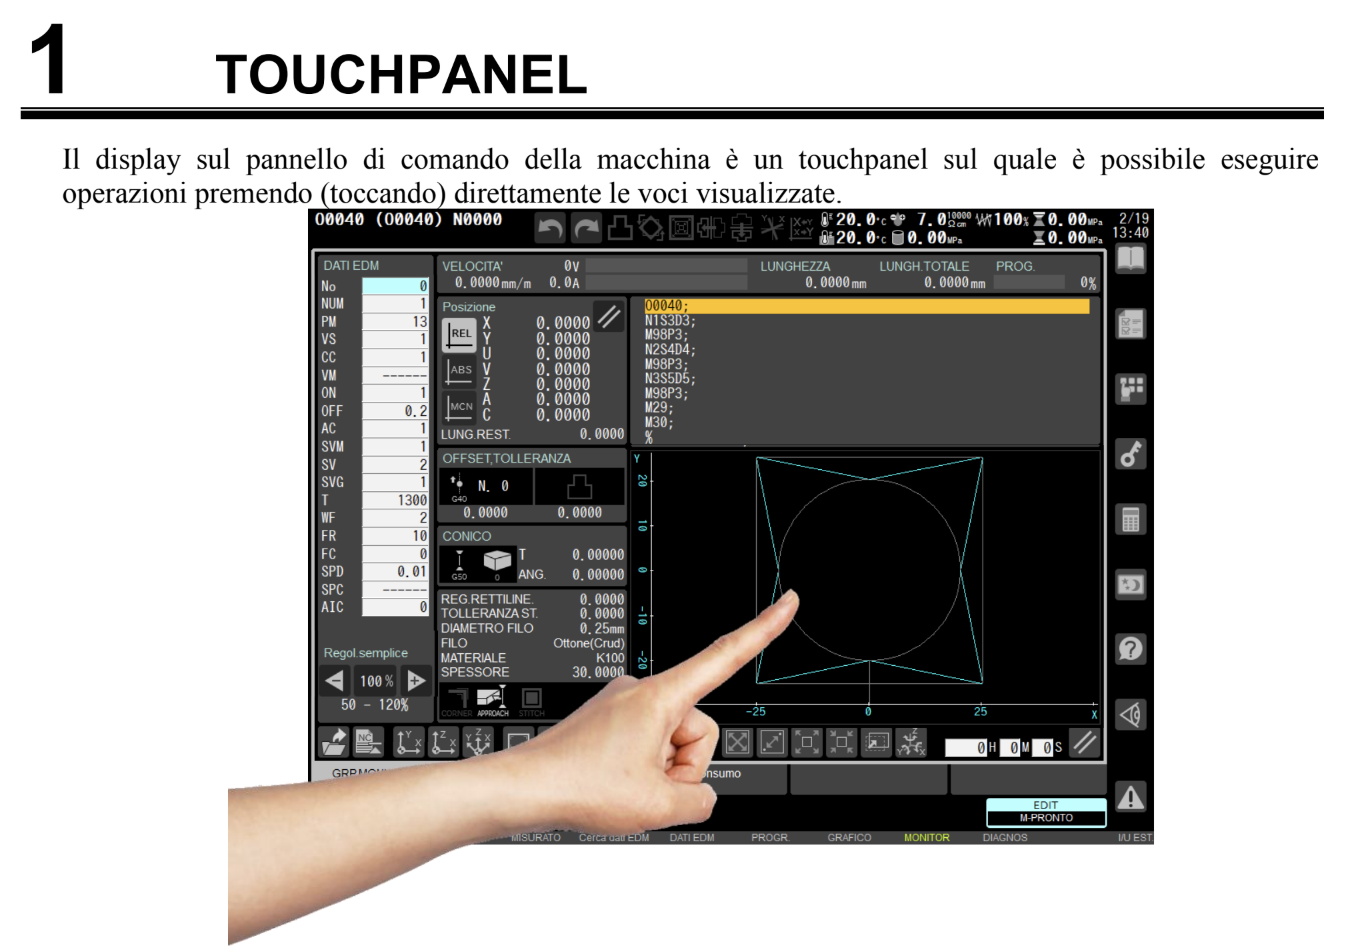
\includegraphics[width=2.5cm,height=1.7cm,keepaspectratio]{figure/asset/touch-panel-schermata-operatore.png}};
\pic[scale=0.7] at (13.25,-1.35) {documento-strutturato};
\node[schema etichetta,text width=2.8cm] at (9.8,-2.7) {\textbf{Ritaglio originale}};
\node[schema etichetta,text width=3.7cm] at (13.25,-2.7)
  {Manuale, pagina ed eventuale caption originale};
\pic[scale=0.67] at (9.4,-4.35) {frammenti};
\node[schema etichetta,text width=3.8cm] at (12.95,-4.35)
  {\textbf{Contesto selezionato}\\Al massimo 6 elementi\\e 2400 caratteri};
\draw[schema freccia] (7,-4.35) -- (8.55,-4.35);
\node[schema nota,text width=6.5cm] at (11.8,-5.45)
  {Il testo serve a disambiguare il visibile.};
\node[schema oggetto,minimum width=2.2cm,minimum height=1.8cm] (vlm) at (9.3,-7.4) {};
\pic[scale=0.8] at (9.3,-7.4) {modello};
\node[schema oggetto,minimum width=2.5cm,minimum height=1.8cm] (descrizione) at (13.1,-7.4) {};
\pic[scale=0.85] at (13.1,-7.4) {dialogo};
\draw[schema freccia] (9.3,-5.95) -- (vlm.north);
\draw[schema freccia] (vlm.east) -- (descrizione.west);
\node[schema etichetta,text width=2.2cm] at (9.3,-8.75) {\textbf{VLM}};
\node[schema etichetta,text width=4.5cm] at (13.1,-8.75)
  {\textbf{Descrizione generata}\\Da confrontare con la fonte};
\pic[scale=0.58] at (0.9,-7.95) {dialogo};
\draw[schemaOcra,line width=1.5pt,line cap=round] (0.25,-8.45) -- (1.55,-7.45);
\node[schema etichetta,anchor=west,align=left,text width=4.8cm] at (2,-8.05)
  {\textbf{Nessun riuso come fonte}\\Le descrizioni generate non entrano nel contesto delle figure successive.};
\end{tikzpicture}
\caption{Composizione degli ingressi del captioning. Le fonti testuali seguono un ordine di priorità, non vengono sommate indiscriminatamente; in assenza di fonti ammissibili, la richiesta non contiene contesto né percorso strutturale. La miniatura dai materiali FANUC forniti è illustrativa, non un risultato del captioning. La descrizione generata va confrontata con la fonte e non diventa una nuova fonte per le richieste successive.}
\label{fig:contesto-caption}
\end{figure}

Il prompt richiede sette campi: \emph{Tipo tecnico}, \emph{Oggetto}, \emph{Elementi visibili}, \emph{Relazioni/funzione}, \emph{Valori/avvertenze}, \emph{Rilevanza RAG} e \emph{Incertezze}. La descrizione deve rimanere entro 1200 caratteri e l'elenco visuale è limitato a otto elementi unici. Le istruzioni impongono di basarsi sul contenuto visibile, di usare il contesto soltanto per disambiguare nomi e sigle, e di dichiarare esplicitamente letture non possibili. Il campo \emph{Rilevanza RAG} richiede una domanda operativa breve, non una misura del recupero. Questi vincoli circoscrivono formato e lunghezza, ma il loro rispetto non prova la fedeltà alla figura. In particolare, il tetto di otto elementi può comprimere eccessivamente tavole esplose o interfacce dense, e quello di 1200 caratteri può escludere una risposta indipendentemente dalla sua qualità informativa.

La scelta finale è il risultato di iterazioni documentate, non di una ricerca di iperparametri su un insieme di test indipendente. Le prove esplorative del settembre 2026 non hanno motivato l'adozione di prompt più lunghi; V3 ha mantenuto il testo del prompt precedente e introdotto controlli aggiuntivi sulle descrizioni. Il successivo ciclo V4 ha escluso le tabelle dalle richieste al VLM, rivisto il contesto delle figure OCR e reso non bloccanti gli errori delle singole caption. Le prove V2 con Ollama \texttt{0.31.2}, le prove intermedie su \texttt{0.33.3} e il ciclo finale su \texttt{0.34.0} devono restare distinti: l'accettazione di un setup storico non si trasferisce automaticamente a quello successivo.

Prima dei controlli, il provider normalizza gli spazi e rimuove le righe vuote della risposta: il limite di lunghezza riguarda il testo normalizzato, non il corpo HTTP grezzo. La risposta viene quindi controllata per formato e lunghezza; alcuni casi richiedono inoltre revisione. Le descrizioni di schemi elettrici e quelle con determinate contraddizioni tra letture incerte e dichiarazioni di assenza di incertezza ricevono lo stato \texttt{review\_required}. La caption viene conservata, ma l'elemento è escluso dall'uso RAG previsto. Un errore di generazione o validazione produce invece \texttt{failed} per l'elemento e una motivazione di esclusione. Gli altri esiti sono \texttt{enriched} e \texttt{skipped}. Il fallimento di una singola caption non coincide necessariamente con l'interruzione dell'intera run.

La provenienza registra provider, modello, versione del prompt, parametri e versione del runtime, oltre a un hash costruito dalla richiesta e dall'asset. È quindi possibile controllare se la descrizione è ancora coerente con gli ingressi documentati. L'hash non certifica che le affermazioni generate siano vere: identifica l'ingresso, non la correttezza semantica dell'uscita.

\subsection{Serializzazione deterministica delle tabelle}

Il modulo \texttt{table\_serialization.py} applica la strategia \texttt{header\_value\_rows\_v1}. Interpreta il contenuto del campo \texttt{table\_markdown}, che può includere rappresentazioni Markdown o HTML, e produce righe testuali con associazioni intestazione--valore. Alla riga vengono aggiunti riferimenti contestuali al manuale, al percorso di capitolo, alla pagina e alla tabella. Non vengono creati chunk né embedding: si prepara una rappresentazione tabellare utilizzabile da componenti successive.

Lo stato \texttt{structured} indica che sono state ottenute righe strutturate; \texttt{fallback} conserva in un'unica riga il contenuto normalizzato quando la struttura non è interpretabile; \texttt{unavailable} indica l'assenza di contenuto tabellare testuale utilizzabile. Quest'ultimo caso può verificarsi anche quando esiste un ritaglio della tabella. La serializzazione non può recuperare valori che il parser non ha acquisito e non usa il VLM per completarli. Mantenere separati questi stati evita di equiparare una tabella trascritta con relazioni esplicite a una semplice conservazione del testo grezzo.

La Figura~\ref{fig:trattamento-visuale} mette a confronto il percorso generativo delle immagini e quello deterministico delle tabelle, mantenendo distinti i rispettivi esiti.

\begin{figure}[!htbp]
\centering
\begin{tikzpicture}[schema base]
\node[schema esterno,text width=13.7cm] at (7.5,0)
  {\textbf{Filtro geometrico comune dopo l'assemblaggio}\\$\rho<0{,}02$: esclusione dall'uso previsto, non cancellazione dell'asset};
\node[schema titolo] at (0.3,-1.3) {Immagini: interpretazione generativa};
\node[schema titolo] at (8.1,-1.3) {Tabelle: trasformazione deterministica};
\draw[schema separatore,draw=schemaGrigio!55] (7.5,-1.6) -- (7.5,-8.55);
\node[schema oggetto,minimum width=4.2cm,minimum height=2.5cm] (immagine) at (3.3,-2.85) {};
\node[inner sep=0pt] at (3.3,-2.6)
  {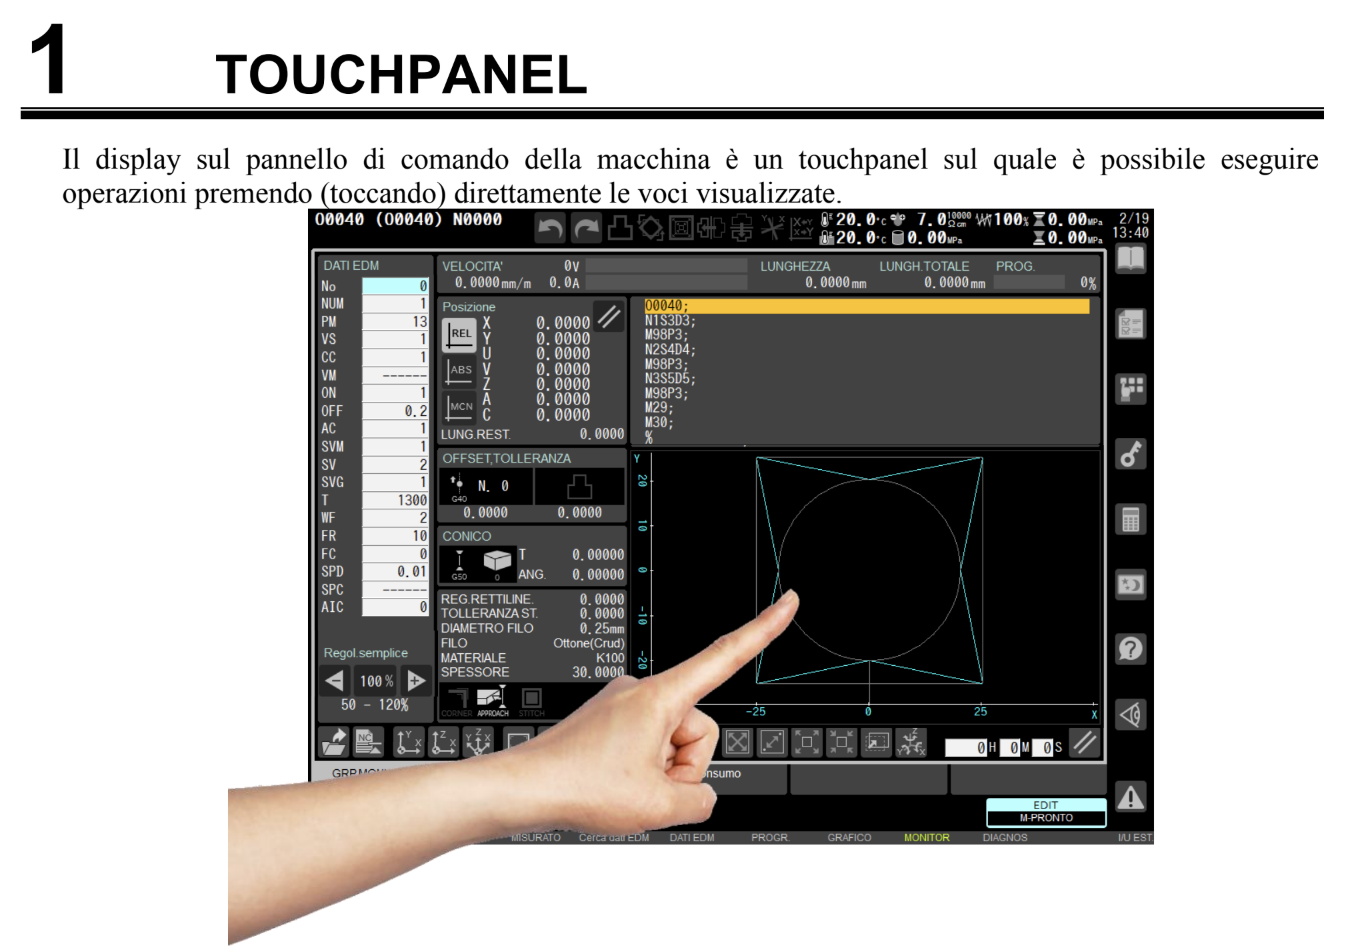
\includegraphics[width=3.7cm,height=2.15cm,keepaspectratio]{figure/asset/touch-panel-schermata-operatore.png}};
\node[schema nota,text width=6cm] at (3.3,-4.05) {Ritaglio ammissibile\\+ eventuale contesto sorgente};
\node[schema oggetto,minimum height=2.5cm] (tabella) at (11.7,-2.85) {};
\pic[scale=1.8] at (11.7,-2.6) {tabella};
\node[schema nota,text width=6cm] at (11.7,-4.05) {Contenuto testuale acquisito\\in Markdown o HTML};
\node[schema oggetto,minimum height=1.5cm] (caption) at (3.3,-5.65) {};
\pic[scale=0.72] at (2.35,-5.65) {modello};
\pic[scale=0.65] at (4.5,-5.65) {dialogo};
\draw[schema freccia] (3.1,-5.65) -- (3.73,-5.65);
\node[schema etichetta,text width=6.1cm] at (3.3,-7.55)
  {\textbf{Captioning con VLM}\\Controlli di formato e lunghezza;\\accettazione, revisione o errore.\\La fedeltà richiede verifica sulla fonte.};
\node[schema oggetto,minimum height=1.5cm] (righe) at (11.7,-5.65) {};
\foreach \ordinata/\colore in {-5.12/schemaBlu,-5.65/schemaVerde,-6.18/schemaOcra} {
  \path[schema icona,draw=\colore,fill=\colore!12] (9.5,\ordinata-0.19) rectangle (13.9,\ordinata+0.19);
  \node[font=\ttfamily\footnotesize] at (11.7,\ordinata) {intestazione: valore};
}
\node[schema etichetta,text width=6.1cm] at (11.7,-7.55)
  {\textbf{Serializzazione delle righe}\\Righe con contesto, testo di ripiego\\o contenuto non disponibile.\\Nessun valore non acquisito viene ricostruito.};
\draw[schema freccia] (3.3,-4.55) -- (caption.north);
\draw[schema freccia] (11.7,-4.55) -- (righe.north);
\end{tikzpicture}
\caption{Trattamento delle immagini e delle tabelle nel workflow corrente; le colonne non indicano esecuzione parallela. Schermata del manuale FANUC dai materiali forniti come esempio visuale, non risultato del captioning; tabella e righe sono schematiche. Le tabelle non vengono inviate al VLM e sono serializzate anche se escluse dall'uso previsto, senza annullare tale esclusione.}
\label{fig:trattamento-visuale}
\end{figure}

\section{Output, tracciabilità e controlli della pipeline}
\label{sec:output-controlli}

\subsection{Artefatti e pubblicazione atomica}

La Tabella~\ref{tab:run-bundle} distingue il documento canonico dagli asset, dai metadati e dalle evidenze di controllo conservati nel bundle.

\begin{table}[!htbp]
\centering
\caption{Artefatti del run bundle nella configurazione ordinaria.}
\label{tab:run-bundle}
\small
\begin{tabularx}{\textwidth}{@{}p{0.27\textwidth}X@{}}
\toprule
Artefatto & Contenuto \\
\midrule
\texttt{manual.json} & Documento canonico: gerarchia, elementi, riferimenti agli asset, descrizioni e tracce. \\
\texttt{toc.json} & Lista delle voci di indice con titolo, livello, pagina ed eventuale confidenza. Non è un indice RAG. \\
\texttt{run.json} & Manifest: identità e stato della run, sorgente e hash, configurazione, capacità rilevate, percorsi, tempi, avvisi ed errori. \tabularnewline
\texttt{validation.json} & Esito dei controlli, messaggi e metriche tecniche; è richiesto nei bundle finali validati o sperimentali. \\
\texttt{assets/} & Rendering e ritagli effettivamente prodotti dagli adattatori. \\
\texttt{diagnostics/} & Evidenze di detection, struttura, filtro, enrichment, runtime e promozione; ulteriori artefatti del percorso OCR. \\
\bottomrule
\end{tabularx}
\end{table}

\texttt{RunBundleWorkspace}, definito in \texttt{run\_bundle.py}, mantiene gli artefatti in una directory di staging sullo stesso filesystem della destinazione. La pubblicazione avviene tramite rinomina dopo il completamento dei controlli. Una destinazione già esistente viene rifiutata, così da non sovrascrivere una run precedente. In caso di errore prima della pubblicazione, lo staging viene rimosso: un insieme incompleto di file non viene presentato come bundle finale.

Il sorgente è identificato mediante nome, dimensione e SHA-256; l'orchestratore verifica che non cambi durante l'elaborazione. I percorsi degli artefatti devono rimanere relativi e non attraversare directory superiori. La diagnostica comune comprende \texttt{detection.json}, \texttt{structure.json}, \texttt{crop\_filter.json}, \texttt{enrichment.json}, \texttt{runtime.json} e \texttt{promotion.json}. Il manifest e la diagnostica registrano configurazioni e versioni necessarie a interpretare la run, ma la riproduzione richiede anche di conservare il PDF identificato e rendere disponibile il runtime corrispondente.

La Figura~\ref{fig:flusso-pubblicazione} segue il passaggio dallo staging al bundle finale e distingue un impedimento alla promozione da un errore che interrompe l'esecuzione. È una vista operativa complementare ai tre piani di verifica della Figura~\ref{fig:livelli-verifica}.

\begin{figure}[!htbp]
\centering
\begin{tikzpicture}[schema base]
\node[schema oggetto,minimum width=2.2cm,minimum height=1.6cm] (inizio) at (1.3,0) {};
\pic[scale=0.76] at (1.3,0) {fascicolo};
\node[schema etichetta,align=left,text width=5.8cm] at (5.85,0)
  {\textbf{Staging: file provvisori}\\Controlli preliminari e detection;\\creazione dello staging\\ed elaborazione};
\node[schema oggetto,minimum width=2.2cm,minimum height=1.6cm] (bozza) at (1.3,-2.5) {};
\pic[scale=0.76] at (1.3,-2.5) {controllo-fonte};
\node[schema etichetta,align=left,text width=5.8cm] (testobozza) at (5.85,-2.5)
  {\textbf{Verifica della bozza}\\Valutazione della promozione;\\scrittura e validazione della bozza};
\node[schema oggetto,minimum width=2.2cm,minimum height=1.6cm] (stato) at (1.3,-5) {};
\pic[scale=0.86] at (1.3,-5) {testo};
\node[schema etichetta,align=left,text width=5.8cm] at (5.85,-5)
  {\textbf{Assegnazione dello stato finale}\\Requisiti soddisfatti: \texttt{validated}\\Impedimenti: \texttt{experimental}};
\node[schema oggetto,minimum width=2.2cm,minimum height=1.6cm] (finale) at (1.3,-7.5) {};
\pic[scale=0.86] at (1.3,-7.5) {checklist};
\node[schema etichetta,align=left,text width=5.8cm] (testofinale) at (5.85,-7.5)
  {\textbf{Controlli finali}\\Manifest finale e report ricalcolato;\\controlli e integrità del sorgente};
\node[schema oggetto,minimum width=2.2cm,minimum height=1.6cm] (pubblicazione) at (1.3,-10) {};
\pic[scale=0.76] at (1.3,-10) {fascicolo};
\path[fill=schemaCartaVerde,draw=schemaVerde] (2.12,-10.42) circle (0.28);
\draw[schemaVerde,line width=1.25pt] (1.96,-10.43) -- (2.07,-10.53) -- (2.29,-10.3);
\node[schema etichetta,align=left,text width=5.8cm] at (5.85,-10)
  {\textbf{Pubblicazione mediante rinomina}\\Bundle \texttt{validated}\\o \texttt{experimental}};
\draw[schema freccia] (inizio) -- (bozza);
\draw[schema freccia] (bozza) -- node[right,schema nota] {Bozza valida} (stato);
\draw[schema freccia] (stato) -- (finale);
\draw[schema freccia] (finale) -- node[right,schema nota] {Controlli superati} (pubblicazione);
\node[schema oggetto,minimum height=1.6cm] (errore) at (12.15,-6) {};
\pic[scale=0.95] at (12.15,-6) {cartella};
\draw[schemaOcra,line width=1.7pt,line cap=round] (11.65,-6.43) -- (12.65,-5.6) (11.65,-5.6) -- (12.65,-6.43);
\node[schema etichetta,text width=4.7cm] at (12.15,-7.65)
  {\textbf{Interruzione}\\Nessun nuovo bundle finale.\\Staging rimosso, se creato.};
\draw[schema freccia] (testobozza.east) -- node[above,schema nota] {Bozza non valida} (15,-2.5) |- (errore.east);
\draw[schema freccia] (testofinale.east) -- (9.65,-7.5) |- node[pos=0.8,above,schema nota] {Errore} (errore.west);
\node[schema nota,text width=4.7cm] at (12.15,-4.2)
  {Anche altri errori fatali possono interrompere il flusso prima della rinomina.};
\node[schema nota,text width=4.7cm] at (12.15,-10)
  {Un errore locale di captioning può essere registrato senza bloccare la pubblicazione.};
\end{tikzpicture}
\caption{Pubblicazione secondo \texttt{orchestrator.py} e \texttt{run\_bundle.py}: dal fascicolo provvisorio a quello pubblicato, oppure all'interruzione. Il segno di spunta indica la pubblicazione, non necessariamente lo stato \texttt{validated}. La conformità tecnica permette di pubblicare; la politica di promozione determina lo stato. I file nello staging sono provvisori fino alla rinomina.}
\label{fig:flusso-pubblicazione}
\end{figure}

\subsection{Validazione tecnica e politica di promozione}

Il validatore in \texttt{validation.py} ricostruisce un report a partire dagli artefatti, invece di fidarsi dell'esito già salvato. Il report dichiarato deve corrispondere a quello ricalcolato; una fingerprint del bundle contribuisce a rilevare modifiche. I controlli riguardano esistenza e schema dei file, coerenza degli identificativi e del sorgente, limiti delle pagine, unicità degli ID, relazioni padre--figlio, percorsi ed esistenza degli asset, provenienza delle caption, struttura della TOC, serializzazione tabellare ed evidenze di promozione.

Un controllo specifico impone che gli elementi canonici coprano almeno il 75\% delle pagine dichiarate elaborate. Indicando con $P$ l'insieme delle pagine elaborate e con $E$ quello delle pagine contenenti almeno un elemento, il requisito è
\begin{equation}
    |E\cap P|\geq\left\lceil0{,}75|P|\right\rceil.
\end{equation}
Questa soglia è distinta da quella usata nella detection: la prima riguarda il risultato del parsing, la seconda il campione testuale di ingresso. Nessuna delle due dimostra che ogni contenuto di una pagina sia stato acquisito, né che tutte le pagine prive di elementi siano effettivamente vuote.

La validazione controlla anche il setup software rispetto alle versioni accettate nella politica implementata. Nelle due run V4 sono registrati Python \texttt{3.12.13}, \texttt{manual\_ingestion 1.0.0}, Pydantic \texttt{2.13.4}, PyMuPDF \texttt{1.28.0} e Pillow \texttt{11.3.0}; la run digitale registra inoltre Docling \texttt{2.112.0}, quella OCR le versioni Paddle indicate nella Sezione~\ref{sec:profili}. Queste identità sono riscontrabili nei manifest e nella diagnostica, ma la versione del pacchetto non identifica da sola ogni revisione dei sorgenti. Il diario riferisce una postazione M1 Max con 32 GB per lo sviluppo; gli artefatti finali non contengono un inventario hardware sufficiente a trattare le durate registrate come un benchmark prestazionale riproducibile su quella configurazione.

La promozione è definita separatamente in \texttt{promotion.py}. Per dichiarare una run \texttt{validated} non basta che il JSON sia leggibile: occorrono copertura dell'intero documento, enrichment conforme, identità coerenti delle caption, assenza di casi che richiedono revisione, assenza di avvisi impeditivi, accettazione del profilo e struttura compatibile con la politica. Per l'OCR la politica registra un identificativo di evidenza di accettazione e distingue la ricostruzione mediante indice dal ripiego sui soli titoli. Nel caso dell'indice stampato OCR, la promozione richiede la risoluzione del 100\% delle righe: la soglia dell'80\% consente alla ricostruzione di proseguire, ma non basta per dichiarare la run validata.

Occorre quindi distinguere tre piani:
\begin{description}
    \item[Conformità tecnica.] Il report assume \texttt{passed} soltanto se tutti i controlli previsti sono superati.
    \item[Stato della run.] Una run tecnicamente coerente è \texttt{experimental} se non soddisfa i requisiti di promozione; è \texttt{validated} quando li soddisfa. Un report \texttt{passed} è compatibile con uno stato \texttt{experimental} correttamente motivato.
    \item[Correttezza semantica.] La fedeltà di testi, gerarchia, ritagli e descrizioni alla fonte richiede un confronto documentale distinto. Non è dimostrata dal nome \texttt{validated}.
\end{description}

I contratti definiscono anche \texttt{incomplete}, \texttt{completed} e \texttt{failed}; il percorso ordinario usa \texttt{completed} per il manifest provvisorio e pubblica l'esito finale soltanto dopo la verifica. Un errore fatale non produce normalmente un bundle finale con stato \texttt{failed}. La CLI può invece scrivere, mediante \texttt{--write-failure-report}, un report compatto accanto alla destinazione, con il contesto dell'interruzione. È quindi necessario raccogliere anche tali esiti quando si valuta la robustezza, evitando di considerare soltanto i bundle pubblicati.

La Figura~\ref{fig:livelli-verifica} riassume la separazione tra conformità tecnica, promozione della run e fedeltà dei contenuti alla fonte. Questa distinzione orienta il metodo di valutazione descritto nel seguito.

\begin{figure}[!htbp]
\centering
\begin{tikzpicture}[schema base]
\node[schema etichetta,text width=14.5cm] at (7.5,1.35)
  {\textbf{Tre domande distinte, non una scala di avanzamento}};
\pic[scale=0.86] at (1.15,0) {checklist};
\node[schema etichetta,anchor=west,align=left,text width=4.35cm] (tecnica) at (2.35,0)
  {\textbf{Conformità tecnica}\\Gli artefatti rispettano il contratto?};
\path[schema icona,fill=white]
  (8.6,-0.82) -- (14.8,-0.82) -- (14.8,0.47) -- (14.45,0.82) -- (8.6,0.82) -- cycle;
\draw[schema icona] (14.45,0.82) -- (14.45,0.47) -- (14.8,0.47);
\node[schema etichetta,text width=5.5cm] (report) at (11.7,0)
  {\textbf{Report} \texttt{passed}\\Tutti i controlli previsti superati};
\draw[schema freccia] (tecnica.east) -- (8.55,0);
\draw[schemaGrigio!45,dash pattern=on 3pt off 4pt,line width=0.65pt] (0,-1.4) -- (15,-1.4);
\pic[scale=0.72] at (1.15,-2.8) {fascicolo};
\node[schema etichetta,anchor=west,align=left,text width=4.35cm] (politica) at (2.35,-2.8)
  {\textbf{Promozione}\\La run soddisfa la politica?};
\node[schema blocco,draw=schemaVerde,fill=schemaCartaVerde,text width=3.5cm,minimum height=0.7cm,inner sep=5pt] (validated) at (12.1,-2.25)
  {\texttt{validated}};
\node[schema esterno,text width=3.5cm,minimum height=0.7cm,inner sep=5pt] (experimental) at (12.1,-3.35)
  {\texttt{experimental}};
\draw[schemaInchiostro,line cap=round] (politica.east) -- (8.25,-2.8);
\draw[schema freccia] (8.25,-2.8) |- node[pos=0.75,above,schema nota] {Sì} (validated.west);
\draw[schema freccia] (8.25,-2.8) |- node[pos=0.75,above,schema nota] {No} (experimental.west);
\draw[schemaGrigio!45,dash pattern=on 3pt off 4pt,line width=0.65pt] (0,-4.25) -- (15,-4.25);
\pic[scale=0.62] at (0.65,-5.7) {pagina};
\pic[scale=0.7] at (1.55,-5.85) {testo};
\draw[schemaBlu,line width=1.15pt] (1.2,-5.65) circle (0.3);
\draw[schemaBlu,line width=1.8pt,line cap=round] (1.42,-5.87) -- (1.78,-6.23);
\node[schema etichetta,anchor=west,align=left,text width=4.35cm] (semantica) at (2.35,-5.7)
  {\textbf{Correttezza semantica}\\Contenuti e associazioni sono fedeli?};
\node[schema etichetta,text width=6.2cm] (fonte) at (11.7,-5.7)
  {\textbf{Confronto documentale con la fonte}\\Non deducibile dagli stati automatici};
\draw[schema freccia] (semantica.east) -- (fonte.west);
\end{tikzpicture}
\caption{Tre domande distinte, non tre tappe equivalenti. La checklist riguarda i controlli tecnici, il fascicolo lo stato della run e la lente il confronto con la fonte. Un report \texttt{passed} è compatibile con una run \texttt{experimental}; nessuno dei due stati dimostra la correttezza semantica.}
\label{fig:livelli-verifica}
\end{figure}

\section{Metodo di valutazione}
\label{sec:valutazione}

La valutazione combina verifica software, prove documentali per profilo e analisi descrittiva dell'enrichment. Non è un benchmark pubblico di parser né uno studio di efficacia del RAG. Le prove complete e le selezioni visuali rispondono a domande diverse: le prime verificano la produzione di una rappresentazione coerente su un intero input; le seconde rendono ispezionabili richieste, informazioni aggiunte ed errori del modello. I test, la matrice di accettazione e le registrazioni finali documentano questo disegno, mantenendo distinta l'evidenza direttamente verificabile da quella conservata soltanto nei report.

La Figura~\ref{fig:metodo-valutazione} organizza le sottosezioni seguenti in un fondamento trasversale e tre assi complementari. La sintesi evita di trattare come fasi consecutive attività che rispondono a domande diverse e usano evidenze differenti.

\begin{figure}[!htbp]
\centering
\begin{tikzpicture}[
  schema base,
  schema asse/.style={schema blocco,minimum width=4.65cm,minimum height=4.9cm,inner sep=8pt},
  schema unita/.style={schema blocco,fill=white,minimum width=1.5cm,minimum height=0.58cm,inner sep=3pt,font=\schemafont\footnotesize},
  schema numero/.style={circle,text=white,font=\schemafont\footnotesize\bfseries,minimum size=7mm,inner sep=0pt},
  schema corpo/.style={font=\schemafont\scriptsize,align=left,text=schemaInchiostro},
  schema rq/.style={circle,draw=schemaBlu,fill=schemaCartaBlu,font=\schemafont\footnotesize\bfseries,minimum size=8mm,inner sep=1pt}
]
\node[schema titolo] at (0,0.45) {Metodo di valutazione: un fondamento comune e tre assi di analisi};

% Fondamento trasversale: definisce che cosa viene contato e dove resta la prova.
\node[schema pannello,minimum width=15cm,minimum height=1.9cm] (fondamento) at (7.5,-0.8) {};
\node[schema numero,fill=schemaBlu] at (0.55,-0.25) {0};
\node[schema titolo] at (0.95,-0.25) {Unità di analisi e registrazioni trasversali};
\node[schema unita] (documento) at (1.25,-1.12) {Documento};
\node[schema unita] (run) at (3.05,-1.12) {Run};
\node[schema unita] (voce) at (4.85,-1.12) {Voce};
\node[schema unita] (elemento) at (6.65,-1.12) {Elemento};
\draw[schema freccia] (documento.east) -- (run.west);
\draw[schema freccia] (run.east) -- (voce.west);
\draw[schema freccia] (voce.east) -- (elemento.west);
\node[schema corpo,anchor=west] at (8.25,-1.02) {%
  \textbf{Tracce conservate}\\
  \texttt{run.json}, snapshot, eventi e asset\\
  richieste e risposte in \texttt{evidence}};

% Tre assi che raggruppano le restanti sottosezioni.
\node[schema asse,draw=schemaVerde,fill=schemaCartaVerde!45] (pipeline) at (2.35,-4.95) {};
\node[schema numero,fill=schemaVerde] at (0.55,-2.95) {1};
\node[schema etichetta,text width=3.6cm] at (2.65,-3.05) {\textbf{Pipeline e struttura}};
\draw[schema tratto,draw=schemaVerde!55] (0.35,-3.55) -- (4.35,-3.55);
\node[schema corpo,anchor=north west] at (0.65,-3.85) {%
  \textbf{Verifica software}\\
  Test e prove di accettazione\\[7pt]
  \textbf{Rappresentazione comune}\\
  Confronto tra struttura,\\
  output e fonte};

\node[schema asse,draw=schemaBlu,fill=schemaCartaBlu!55] (studio) at (7.5,-4.95) {};
\node[schema numero,fill=schemaBlu] at (5.7,-2.95) {2};
\node[schema etichetta,text width=3.6cm] at (7.8,-3.05) {\textbf{Studio V4 sull'enrichment}};
\draw[schema tratto,draw=schemaBlu!55] (5.5,-3.55) -- (9.5,-3.55);
\node[schema corpo,anchor=north west] at (5.8,-3.85) {%
  \textbf{Disegno V4}\\
  Selezione mirata e campione\\[5pt]
  \textbf{Confronto descrittivo}\\
  Baseline, output e giudizio\\[5pt]
  \textbf{Misure operative}\\
  Esclusioni e denominatori\\
  Durate registrate};

\node[schema asse,draw=schemaOcra,fill=schemaCartaGialla!55] (audit) at (12.65,-4.95) {};
\node[schema numero,fill=schemaOcra] at (10.85,-2.95) {3};
\node[schema etichetta,text width=3.6cm] at (12.95,-3.05) {\textbf{Audit e riproducibilità}};
\draw[schema tratto,draw=schemaOcra!65] (10.65,-3.55) -- (14.65,-3.55);
\node[schema corpo,anchor=north west] at (10.95,-3.85) {%
  \textbf{Catena verificata}\\
  Asset e richiesta\\
  Risposta e documento finale\\[7pt]
  \textbf{Integrità e identità}\\
  Hash, fingerprint e sorgenti\\[7pt]
  \textbf{Riproducibilità}\\
  Revisione eseguita\\
  non riproducibile integralmente};

% Il fondamento comune alimenta tutti gli assi; ciascun asse sostiene una RQ.
\coordinate (dorsale-sinistra) at (2.35,-2.08);
\coordinate (dorsale-centro) at (7.5,-2.08);
\coordinate (dorsale-destra) at (12.65,-2.08);
\draw[schema tratto,draw=schemaInchiostro,line width=0.8pt]
  (fondamento.south) -- (dorsale-centro);
\draw[schema tratto,draw=schemaInchiostro,line width=0.8pt]
  (dorsale-sinistra) -- (dorsale-destra);
\fill[schemaInchiostro] (dorsale-sinistra) circle (1.15pt);
\fill[schemaInchiostro] (dorsale-centro) circle (1.15pt);
\fill[schemaInchiostro] (dorsale-destra) circle (1.15pt);
\draw[schema freccia] (dorsale-sinistra) -- (pipeline.north);
\draw[schema freccia] (dorsale-centro) -- (studio.north);
\draw[schema freccia] (dorsale-destra) -- (audit.north);

\node[schema rq] (rqone) at (2.35,-8.1) {RQ1};
\node[schema rq] (rqtwo) at (7.5,-8.1) {RQ2};
\node[schema rq] (rqthree) at (12.65,-8.1) {RQ3};
\draw[schema freccia] (pipeline.south) -- (rqone.north);
\draw[schema freccia] (studio.south) -- (rqtwo.north);
\draw[schema freccia] (audit.south) -- (rqthree.north);
\end{tikzpicture}
\caption{Organizzazione del metodo di valutazione. Le unità e le registrazioni sono trasversali; le altre sottosezioni confluiscono in tre assi complementari, rispettivamente collegati alla rappresentazione comune, all'enrichment V4 e alla verificabilità degli artefatti.}
\label{fig:metodo-valutazione}
\end{figure}
\FloatBarrier

\subsection{Unità di analisi e registrazione delle esecuzioni}

Si distinguono quattro unità: documento, run, voce gerarchica ed elemento. Il documento identifica la fonte; la run identifica una particolare elaborazione e configurazione; la voce gerarchica consente di verificare titolo, livello, destinazione e relazione con il padre; l'elemento consente di controllare acquisizione, appartenenza, asset ed eventuali informazioni derivate. Ripetizioni o prove parziali sullo stesso PDF non devono essere conteggiate come documenti indipendenti.

Per le run V4 questi dati sono conservati in \texttt{run.json}, \texttt{validation.json} e nella directory \texttt{evidence}. Quest'ultima registra comando e argomenti effettivi, configurazione del provider, esito della CLI, eventi temporali, chiamate di enrichment e scambi HTTP. Le snapshot \texttt{manual-before.json} e \texttt{manual-after.json} delimitano la trasformazione generativa; l'inventario degli asset e gli hash consentono di collegare la richiesta al ritaglio effettivamente inviato. Il conteggio delle chiamate proviene dalle registrazioni, non dal solo numero di caption presenti nel documento finale.

Le esecuzioni senza provider e quelle su un sottoinsieme delle pagine restano identificate come diagnostiche. L'unità per descrivere l'esito della pipeline è il tentativo di esecuzione, inclusi eventuali fallimenti senza pubblicazione; l'unità per descrivere il captioning è la singola richiesta al provider. Gli esiti delle prove esplorative V3 non sono aggregati a quelli del ciclo V4: il comportamento sugli errori e il trattamento delle tabelle sono cambiati. L'archivio V4 documenta due tentativi, non il totale di tutte le prove svolte durante lo sviluppo.

\subsection{Verifica software e prove di accettazione}

La directory \texttt{tests} contiene 22 moduli di test. La loro funzione è verificare contratti e transizioni osservabili, anche con PDF sintetici, provider simulati e risposte OCR controllate; non attribuire accuratezza semantica ai motori reali. La Tabella~\ref{tab:test-metodi} riassume le aree pertinenti al metodo. La matrice storica registra una suite di 329 test superati per il rilascio allora verificato: quel conteggio non viene trasferito automaticamente allo stato dei sorgenti qui archiviati, né presentato come una nuova esecuzione della suite.

\begin{table}[!htbp]
\centering
\caption{Copertura funzionale dei test in \texttt{tesi-di-nardo/tests}, distinta dalla verifica semantica del corpus.}
\label{tab:test-metodi}
\small
\begin{tabularx}{\textwidth}{@{}>{\raggedright\arraybackslash}p{0.25\textwidth}X@{}}
\toprule
Area & Comportamenti verificati dai test presenti \\
\midrule
Detection e profili & Routing, input inutilizzabili, scelta del parser e rifiuto di override incoerenti. \tabularnewline
Struttura & Offset, indice multipagina, titoli lunghi o duplicati, limiti di pagina, ancoraggi locali e ricostruzione OCR. \tabularnewline
Asset ed enrichment & Percorsi, filtro, fonti immutabili, esclusione delle tabelle dal VLM, provenienza e risposte non conformi. \tabularnewline
Tabelle & Markdown/HTML, celle unite, intestazioni irregolari, fallback e testo assente; purezza, determinismo e idempotenza. \tabularnewline
Orchestrazione e bundle & Pubblicazione atomica, protezione dalla sovrascrittura, integrità, report, promozione e fallimenti. \tabularnewline
\bottomrule
\end{tabularx}
\end{table}

Due test rendono esplicite le scelte finali dell'enrichment: il primo usa un provider che genera un errore se chiamato su una tabella, verificando che la tabella lo salti; il secondo costruisce una pagina con sezioni relative a figure diverse e verifica che il prompt usi soltanto il testo associato alla figura bersaglio. Queste prove isolano il comportamento voluto, ma non stabiliscono quanto spesso il riconoscimento del contesto riesca sui PDF reali. Analogamente, i test della serializzazione verificano la trasformazione delle celle già acquisite, non la correttezza dell'OCR che le ha prodotte.

\subsection{Verifica della rappresentazione comune}

Per il profilo digitale ricostruito il riferimento del confronto è l'outline del PDF gemello. La matrice riporta un confronto su titoli, pagine, ordine e livelli, con una correzione esplicita dell'offset di livello alla radice. Recall e precision dei titoli descrivono copertura e sovrapproduzione rispetto a quel riferimento; la corrispondenza di pagina è distinta fra esatta ed entro una pagina di scarto. Il benchmark riguarda la gerarchia, non misura automaticamente la conservazione del testo o l'associazione delle figure ai capitoli. L'harness di confronto e le corrispondenze elementari non sono inclusi nell'archivio del progetto: i punteggi restano quindi quelli delle prove storiche, senza un nuovo calcolo.

Per l'OCR, la prova integrale documentata considera l'indice stampato a pagina 5 del WM250, lo scarto tra numerazione stampata e pagina fisica e la risoluzione delle relative voci. La matrice descrive anche l'ispezione delle pagine 26 e 33, ruotate di 180 gradi, insieme ai ritagli. Si tratta di verifiche localizzate, non di una trascrizione di riferimento completa del manuale. La run V4 sulle sole pagine 8, 10, 26 e 33 non comprende l'indice a pagina 5 e usa il fallback sui titoli OCR: il suo limite strutturale non va confuso con l'esito del percorso completo mediante indice.

La verifica semantica ha come riferimento la fonte visuale, non il solo JSON. Per gli elementi si distinguono conservazione del testo, completezza del ritaglio, associazione al capitolo e ordine di lettura. Il confronto deve essere bidirezionale: partire dall'output permette di individuare contenuti errati o duplicati, ma solo partire dalla pagina sorgente consente di rilevare omissioni. Poiché l'archivio del progetto non include i PDF integrali, il confronto sui ritagli digitali riguarda le figure conservate e lascia aperta la verifica di eventuali omissioni nelle pagine originarie. Per la selezione OCR sono invece conservati anche i rendering delle quattro pagine.

Le tabelle richiedono un confronto tra celle della fonte, rappresentazione acquisita e righe serializzate. È necessario distinguere errori già introdotti dal parser da errori di serializzazione; il ricalcolo deterministico controlla la seconda trasformazione, non la trascrizione originaria. Analogamente, per le figure bisogna separare ritagli errati, contesti errati e descrizioni errate, poiché si tratta di difetti di stadi differenti.

Le tabelle reali appartengono alle prove storiche complete e alle selezioni delle pagine 3 e 1004, non al campione visuale finale V4. Il confronto riportato nella matrice distingue struttura disponibile, fallback e contenuto testuale assente; non giustifica l'attribuzione di accuratezza cella per cella all'intero corpus. La disponibilità dei test e dei conteggi storici permette di documentare il metodo di serializzazione, senza presentare i due bundle V4, privi di elementi \texttt{table}, come una nuova prova empirica di tale componente.

\subsection{Disegno e campione dello studio finale V4}

Lo studio V4 adotta una selezione mirata e descrittiva di contenuti reali, non un campionamento casuale. Il diario del 15 settembre 2026 stabilisce un ciclo digitale con outline e uno scansionato, senza replicare le immagini digitali nel profilo ricostruito. Le pagine effettivamente elaborate e la popolazione visuale risultante sono ricostruibili dai comandi, dalle snapshot e dai report del filtro, come sintetizzato nella Tabella~\ref{tab:campione-v4}.\footnote{I comandi e gli ingressi effettivi sono conservati nei due file \path{evidence/command.json}; i conteggi sono riscontrabili in \path{bundle/diagnostics/crop_filter.json} e nelle directory \path{evidence/captions}, sotto ciascun caso in \path{tesi-di-nardo/enrichment-v4-final-20260915}.}

\begin{table}[!htbp]
\centering
\caption{Formazione del campione V4: il filtro esclude immagini prima della generazione, non in seguito a errori del VLM. Le selezioni non contengono elementi canonici di tipo tabella.}
\label{tab:campione-v4}
\small
\begin{tabularx}{\textwidth}{@{}>{\raggedright\arraybackslash}p{0.17\textwidth}Xrrr@{}}
\toprule
Caso & Pagine PDF elaborate & Immagini & \shortstack{Escluse\\dal filtro} & Chiamate \tabularnewline
\midrule
Digitale con outline & 73, 93, 98, 225, 228, 352 & 16 & 7 & 9 \\
Scansione WM250 & 8, 10, 26, 33 & 9 & 1 & 8 \\
\midrule
Totale & 10 pagine su due documenti & 25 & 8 & 17 \\
\bottomrule
\end{tabularx}
\end{table}

Il caso digitale è registrato come \path{enrichment-v4-outline-20260915}; quello scansionato come \path{enrichment-v4-scanned-20260915}. Nel digitale il campione comprende uno schema di collegamento elettrico, il touch panel, la tastiera di movimento e schermate o barre di navigazione dell'interfaccia. Nello scansionato comprende fotografie di gruppi meccanici e comandi, oltre a due tavole esplose. Queste classi sono ricavabili dai ritagli; non vengono dedotte dall'etichetta \emph{Tipo tecnico} generata dal modello, che può essere errata.

Le 17 richieste riguardano 17 asset con digest distinti. La selezione mira a rendere osservabili contenuti spaziali, sigle, comandi e relazioni fra figura e testo, senza pretese di rappresentatività statistica dei manuali. Le pagine sono fissate prima delle due esecuzioni documentate, ma provengono da un percorso di sviluppo che ha già utilizzato materiali dello stesso progetto: non costituiscono un insieme di test indipendente dalle scelte di prompt e filtro. Ogni richiesta dispone di una sola risposta nel ciclo archiviato; non sono previste repliche da cui stimare la variabilità della generazione.

\subsection{Baseline e confronto descrittivo}

La baseline è la rappresentazione acquisita prima dell'enrichment: testo della pagina, eventuale \texttt{caption\_original}, collegamenti documentali e asset. Non è una risposta di un sistema RAG alternativo. Nelle nove immagini digitali inviate al modello la caption originale è assente, ma esiste testo contestuale nelle pagine; nelle immagini OCR possono essere già presenti sigle o frammenti di testo riconosciuti. La baseline comprende quindi anche informazioni testuali sulla figura disponibili al di fuori della caption originale. La snapshot \texttt{manual-before.json} e il prompt effettivo permettono di distinguere ciò che è già disponibile da ciò che viene aggiunto dalla lettura visuale.

Il confronto descrittivo documentato nel diario affianca originale, baseline, output Qwen e giudizio breve. Nella valutazione si distinguono: aggiunte visuali supportate dalla fonte; ripetizioni di informazioni già disponibili; omissioni; dettagli o relazioni non supportati; letture errate di sigle e valori; dichiarazioni di incertezza. Non vengono introdotti punteggi di qualità aggregati né un beneficio netto presunto. Le registrazioni tecniche consentono di ricostruire i primi tre termini del confronto; le schede qualitative curate richiamate dal diario non sono comprese nell'archivio del progetto. La documentazione conservata non specifica un protocollo di annotazione indipendente con numero di revisori, accordo inter-annotatore o risoluzione dei disaccordi.

Una caption più lunga o accettata dal validatore non è, per questo, migliore. Analogamente, \texttt{review\_required} è l'esito di una regola automatica che segnala la necessità di controllo, non la prova che un revisore umano sia intervenuto. Per separare i livelli di errore, l'analisi distingue ritaglio sbagliato, contesto non pertinente e interpretazione inesatta di un ingresso corretto. Un'informazione presente nel contesto ma non visibile può spiegare l'uscita del modello senza renderla una lettura fedele della figura.

\subsection{Esclusioni, denominatori e misure operative}

I denominatori dipendono dallo stadio. Per descrivere il filtro si considerano tutte le 25 immagini acquisite; per descrivere la generazione si considerano le 17 chiamate effettive, comprese quelle la cui risposta non entra nel documento finale. Le immagini escluse prima della chiamata, quelle fallite e quelle da rivedere devono rimanere categorie separate. La conservazione degli scarti consente di valutare anche informazione utile eventualmente sottratta all'uso successivo, anziché limitarsi ai casi accettati.

Le risposte oltre il limite di lunghezza sono conservate in \texttt{caption-response.json} e nei corpi delle risposte HTTP anche quando \texttt{caption\_generated} resta vuoto nel documento. Limitare la revisione alle sole caption finali introdurrebbe quindi una selezione favorevole degli esiti. Viceversa, le caption da rivedere possono rimanere nel documento ma con \texttt{include\_in\_rag=false}, che ne mantiene esplicita l'esclusione dall'uso previsto.

Gli eventi e i file \texttt{call.json} distinguono durata della CLI, durata dell'enrichment e durata delle richieste al provider. Un tempo totale include anche acquisizione, rendering, controlli e registrazione degli artefatti; non può essere attribuito integralmente al modello. Le durate disponibili descrivono due esecuzioni strumentate, con diverso numero di pagine e parser: non supportano confronti di velocità fra motori né stime di throughput generalizzabili. Gli esiti operativi e gli esempi di contenuto sono destinati al Capitolo~\ref{cap:risultati}, mantenendo separati metodo e risultati.

\subsection{Audit degli artefatti e limiti di riproducibilità}
\label{sec:audit-metodi}

L'audit dei materiali V4 verifica la catena \emph{asset--richiesta--risposta--documento}. Per ciascuna chiamata sono confrontati il digest del ritaglio, quello dell'immagine codificata nel corpo HTTP e il prompt salvato. Per le caption dotate di provenance si ricostruisce l'hash dall'identificativo dell'elemento, dal tipo, dal prompt e dai byte dell'asset. Si controllano inoltre gli inventari delle immagini e la corrispondenza fra snapshot dopo l'enrichment e documento finale. Poiché i due campioni non contengono tabelle, questa corrispondenza non è una prova della serializzazione tabellare.

La fingerprint del bundle viene ricalcolata su nomi relativi e contenuto di tutti i file, escludendo \texttt{validation.json}, che conserva il valore atteso. In entrambi i casi coincide con quella archiviata. I report salvati dichiarano 30 controlli superati, mentre i manifest riportano \texttt{experimental}. Questa combinazione è coerente con il significato degli stati: il ciclo è parziale e conserva limitazioni dell'enrichment, oltre al fallback strutturale nel caso OCR. Il ricalcolo verifica l'integrità del bundle rispetto all'impronta registrata; in questo controllo non vengono rieseguiti il validatore completo o l'ingestion.

Un secondo controllo riguarda \texttt{source-hashes.json}. Per ciascuna run sono registrati 34 sorgenti del pacchetto: 32 corrispondono byte per byte ai file conservati nell'archivio del progetto, mentre \texttt{enrichment.py} e \texttt{orchestrator.py} hanno digest diversi. L'inventario cita inoltre lo script sperimentale \texttt{final\_run.py}, il protocollo e \texttt{pyproject.toml}, assenti dall'archivio.\footnote{Inventari conservati in \path{tesi-di-nardo/enrichment-v4-final-20260915/outline/evidence/source-hashes.json} e nel corrispondente caso \texttt{scanned}; il prefisso storico \texttt{src/} è ricondotto al pacchetto \texttt{manual\_ingestion} qui archiviato.} Nella descrizione si distinguono quindi la revisione eseguita, il cui comportamento è documentato dagli artefatti della run, e l'implementazione corrente, descritta attraverso il codice e i test. La differenza tra i sorgenti limita la riproduzione esatta finché non è disponibile la revisione corrispondente, pur lasciando verificabile l'integrità dei bundle conservati.

Per ripetere integralmente lo studio occorrono i PDF identificati dagli hash, i sorgenti della revisione eseguita, lo script di strumentazione e i runtime registrati. La matrice segnala inoltre che le dipendenze transitive Python non sono congelate per hash. L'archiviazione di parametri, input e risposte permette dunque un audit sostanziale del ciclo conservato, ma non va confusa con una riproducibilità completa già dimostrata in un ambiente indipendente.

La Tabella~\ref{tab:rq-evidenze} collega le domande di ricerca alle evidenze disponibili e ai loro limiti.

\begin{table}[!htbp]
\centering
\caption{Domande di ricerca e livelli di evidenza. Le fonti storiche e gli artefatti direttamente ispezionabili mantengono ruoli distinti.}
\label{tab:rq-evidenze}
\small
\begin{tabularx}{\textwidth}{@{}p{0.12\textwidth}XX@{}}
\toprule
Domanda & Evidenze utilizzate & Distinzione da mantenere \\
\midrule
RQ1 & Matrice dei tre profili, test strutturali, TOC e documenti V4. & Prove complete storiche, selezioni finali e correttezza semantica delle associazioni. \tabularnewline
RQ2 & Asset, baseline e 17 richieste/risposte V4; prove storiche e test tabellari. & Aggiunte, omissioni ed errori; generazione e serializzazione; limiti dell'analisi qualitativa. \tabularnewline
RQ3 & Manifest, provenienza, report, fingerprint e registrazioni delle chiamate. & Integrità dei bundle, promozione, identità dei sorgenti e validazione semantica. \tabularnewline
\bottomrule
\end{tabularx}
\end{table}

La validità delle conclusioni resta circoscritta ai due manuali di base, alle condizioni di ingresso e alle selezioni effettivamente documentate. Un bundle strutturato e verificabile può costituire un ingresso per un sistema RAG. Gli eventuali effetti su retrieval, generazione, sicurezza operativa e carico di lavoro richiederebbero una valutazione downstream distinta, esterna ai controlli documentali svolti in questo studio.